\chapter{Proportionnalité} \label{Tra8}

\begin{prerequis}[Dans les programmes - cycle 3]
   {\bf Résoudre des problèmes en utilisant des fractions simples, les nombres décimaux et le calcul.}
   \begin{itemize}
      \item Reconnaître et résoudre des problèmes relevant de la proportionnalité en utilisant une procédure adaptée : propriétés de linéarité (additive et multiplicative), passage à l’unité, coefficient de proportionnalité. \\
      Appliquer un pourcentage. \\
      \ \\
      \ \\
   \end{itemize}
   {\bf Résoudre des problèmes impliquant des grandeurs (géométriques, physiques, économiques) en utilisant des nombres entiers et des nombres décimaux.}
   \begin{itemize}
      \item Identifier une situation de proportionnalité entre deux grandeurs à partir du sens de la situation. Résoudre un problème de proportionnalité impliquant des grandeurs.
   \end{itemize}
   {\bf Reconnaitre et utiliser quelques relations géométriques}
   \begin{itemize}
      \item Reproduire une figure en respectant une échelle donnée. \\
      Agrandissement ou réduction d’une figure.
   \end{itemize}
\end{prerequis}


%%%%%%%
\reperes %%%
%%%%%%%

%%%%%%%%%%%%%%%%%%%%%%%%%%%%%%%%
\section{Repères de progressivité et stratégies d'enseignement}
%%%%%%%%%%%%%%%%%%%%%%%%%%%%%%%%

Dans les programmes de 2008, la proportionnalité apparaît à part entière dans le thème \og Organisation et gestion de données \fg{}. Ce thème ayant disparu des nouveaux programmes de 2015 en tant que tel, la proportionnalité se traite en fil rouge dans les trois domaines que sont \og Nombres et calculs \fg, \og Espace et géométrie \fg, et \og Grandeurs et mesures \fg{} [edu3]. \medskip

La résolution de problèmes de proportionnalité est un terrain particulièrement fécond pour les interactions entre la langue française et le langage mathématique puisque la verbalisation en langage naturel des procédures utilisées (prendre le double, le triple, le tiers, le quadruple, d’une grandeur) contribue à la fois à l’élargissement du répertoire lexical et à et la compréhension d’une notion mathématique. \\
Sa maîtrise est essentielle tant pour un usage dans la vie courante que dans un cadre professionnel. Son apprentissage s’inscrit dans la durée. \medskip

Les premiers problèmes de proportionnalité rencontrés sont des problèmes de multiplication et des problèmes de division (\og un ballon de foot pèse 450 g, combien pèsent 3 ballons de foot identiques ? \fg). Proposés dès le CE1, ils sont résolus à l'aide de procédures personnelles et préparent les élèves à la reconnaissance de situations de proportionnalité. C'est à partir du CM1 que le langage spécifique de proportionnalité apparait : \\
{\bf -- Au CM1}, dès la P1, des situations de proportionnalité peuvent être proposées (recettes\dots). Le recours aux propriétés de linéarité (multiplicative et additive) est privilégié. Ces propriétés doivent être explicitées ; elles peuvent être institutionnalisées de façon non formelle à l’aide d’exemples verbalisés (\og si j’ai deux fois, trois fois… plus d’invités, il me faudra deux fois, trois fois… plus d’ingrédients \fg ; \og si 6 stylos coutent 10 euros et 3 stylos coutent 5 euros, alors 9 stylos coutent 15 euros \fg). \\
L'institutionnalisation des propriétés se fait progressivement à partir de la P2. \\
{\bf -- Au CM2}, dès la P1, le passage par l’unité vient enrichir la palette des procédures utilisées lorsque cela s’avère pertinent. à partir de la P3, le symbole \% est introduit dans des cas simples, en lien avec les fractions d’une quantité (50\% pour la moitié ; 25\% pour le quart ; 75\% pour les trois quarts ; 10\% pour le dixième). \\
Des situations très simples impliquant des échelles et des vitesses constantes peuvent également être rencontrées : les élèves agrandissent ou réduisent une figure dans un rapport simple donné (par exemple $\times\frac12, \times2$ ou $\times3$). Si le coefficient de proportionnalité est rencontré au cours moyen, notamment lors de travaux sur les échelles, son institutionnalisation dans un cadre général peut être reportée en toute fin de cycle 3. \\

{\bf\large Stratégies d'enseignement} \\ [1mm]
Pour que la proportionnalité prenne tout son sens, l’élève doit être confronté à des situations ne relevant pas de la proportionnalité (\og Si je mesure 1 mètre à 10 ans, je peux mesurer 2 mètres à 20 ans mais pas 4 mètres à 40 ans \fg). \\
Les propriétés de linéarité pour l’addition et pour la multiplication par un nombre doivent être le plus souvent possible explicitées. L’enseignant propose dans un premier temps des situations mettant en jeu des nombres entiers entretenant entre eux des rapports simples (double, triple, quintuple, etc.) pour aller progressivement vers des situations plus compliquées (nombres décimaux, fractions, rapports plus complexes). \\ [1mm]
Les {\bf tableaux de proportionnalité} ne doivent pas être conçus comme des objets d’enseignement ; s’ils peuvent permettre de résumer clairement une situation proposée dans un problème, les opérations à réaliser pour résoudre un problème de proportionnalité au cycle 3 ne doivent pas se faire par un raisonnement sur des lignes ou des colonnes d’un tableau mais uniquement sur des cardinaux ou des grandeurs, en explicitant ce qui est fait, tant à l’oral qu’à l’écrit. En variant les nombres et les relations numériques, l’enseignant habitue l’élève à changer de procédure pour choisir de manière pertinente la plus efficace pour lui.


%%%%%%%%%%%%%%%%%%%%%%%
\section{Les procédures de résolution à l'école} 
%%%%%%%%%%%%%%%%%%%%%%%
 
Au niveau de l'école primaire, on utilise essentiellement les propriétés de linéarité (additive, multiplicative ou mixte), ainsi que le passage à l'unité et le coefficient de proportionnalité dans des cas simples. L’objectif n’est pas, à ce stade, de mettre en avant telle ou telle procédure particulière, mais de permettre à l’élève de disposer d’un répertoire de procédures, s’appuyant toujours sur le sens, parmi lesquelles il pourra choisir en fonction des nombres en jeu dans le problème à résoudre. Chaque méthode devra être réinvestie dans les trois registres numérique - grandeurs - géométrique. \\

{\bf Procédure utilisant la propriété de linéarité additive.}
\begin{center}
{\renewcommand{\arraystretch}{1.2}
\begin{tabular}{|p{7cm}|p{7cm}|}
   \hline
   \cellcolor{FondTableaux}{Nombres et calculs} & \cellcolor{FondTableaux}{Grandeurs et mesures} \\
   \hline
   On souhaite calculer $7\times12$. \newline
   $\bullet$ $7\times10 =70$ ; \newline
   $\bullet$ $7\times2 =14$ ; \newline
   $12 =10+2$ donc, par linéarité additive : \newline
   $7\times12 =70+14 =84$.
   &
   3 kg de letchis coûtent 3,60 \euro ; \newline
   5 kg de letchis coûtent 6 \euro{} ; \newline
   8 kg de letchis coûtent 3,60 \euro{} + 6 \euro{} = 9,60 \euro. \\
   \hline 
\end{tabular}}
\end{center}

\smallskip

{\bf Procédure utilisant la propriété de linéarité multiplicative.}
\begin{center}
{\renewcommand{\arraystretch}{1.2}
\begin{tabular}{|p{7cm}|p{7cm}|}
   \hline
   \cellcolor{FondTableaux}{Grandeurs et mesures} & \cellcolor{FondTableaux}{Espace et géométrie} \\
   \hline
   Une douzaine d'oeufs identiques pèsent 600 g \newline
   donc, par linéarité multiplicative : \newline\
   $\bullet$ 6 oeufs pèsent deux fois moins, soit 300 g ; \newline
   $\bullet$ 36 oeufs pèsent trois fois plus, soit 1 800 g. 
   &
   Mon triangle a pour mesures 3 cm, 4 cm et 5 cm. \newline\
   J'effectue un agrandissement pour que le côté le plus grand mesure 20 cm. \newline
   Il s'agit d'un agrandissement de facteur 4, donc, les deux autres côtés mesurent respectivement 12 cm et 16 cm. \\
   \hline 
\end{tabular}}
\end{center}

\smallskip

{\bf Autres procédures.}

Une fois ces deux procédures fondamentales parfaitement assimilées, on peut entrer dans des problèmes de proportionnalité un peu plus complexes. Imaginons par exemple le problème suivant donné à des élèves de cycle 3 : \\
\og {\it Axel a acheté 6 stylos tous identiques et au même prix. Il a payé 9 \euro. Combien aurait-il payé si il en avait acheté 15 ?} \fg. 

\begin{center}
{\renewcommand{\arraystretch}{1.2}
\begin{tabular}{|p{4.5cm}|p{4.5cm}|p{4.5cm}|}
   \hline
   \cellcolor{FondTableaux}{Linéarité mixte} & \cellcolor{FondTableaux}{Passage par l'unité} & \cellcolor{FondTableaux}{\small Coefficient de proportionnalité} \\
   \hline
   15 stylos = 12 stylos + 3 stylos ; \newline
   6 stylos coûtent 9 \euro ; \newline
   $\bullet$ 12 stylos coûtent 18 \euro ; \newline
   \hspace*{0.1cm} (deux fois plus) ; \newline
   $\bullet$ 3 stylos coûtent 4,5 \euro \newline
   \hspace*{0.1cm} (la moitié) ; \newline
   15 stylos coûtent 22,5 \euro \newline
   (18 \euro{} + 4,5 \euro{} = 22,5 \euro).
   &
    6 stylos coûtent 9 \euro ; \newline
   $\bullet$ 1 stylo coûte 1,5 \euro ;
   \hspace*{0.1cm} ($9\text{ \euro}\div6$) \newline
   15 stylos coûtent 22,5 \euro{} \newline
   ($15\times1,5$ \euro{} = 22,5 \euro).
   &
   6 stylos coûtent 9 \euro ; \newline
   le coefficient de proportionnalité permettant de passer de 6 à 9 est de 1,5 ($6\times1,5 =9$) ; \newline
   15 stylos coûtent 22,5 \euro \newline
   ($15\times1,5 =22,5$). \\
   \hdashline
   + Méthode de calcul mental.\newline
   + Facile à comprendre. \newline
   -- Peut être long.
   &
   + Méthode ayant du sens. \newline
   -- Arrondis parfois source d'erreur.
   &
   + Méthode rapide. \newline
   -- Coefficient difficile à trouver. \newline
   -- Moins intuitif. \\
   \hline
\end{tabular}}
\end{center}

\section{Typologie des problèmes posés}%%%%%%%%%%%

On peut classer les problèmes de proportionnalité en plusieurs catégories.

\bm{Problèmes de recherche d'un 4\up{ème} proportionnelle} : trois données sont connues, et on recherche la quatrième, ce sont les problèmes les plus classiques pouvant porter sur des grandeurs de même nature ou de nature différente.
   
\begin{center}
{\renewcommand{\arraystretch}{1.2}
\begin{tabular}{|p{7cm}|p{7cm}|}
   \hline
   \cellcolor{FondTableaux}{Grandeurs de même nature}
   &
   \cellcolor{FondTableaux}{Grandeurs de nature différente} \\
   \hline
   Sur une carte de la Réunion, 5 cm représentent 10 km dans la réalité. Pour aller de Saint-Denis à Saint-Pierre, on trouve 35 cm sur la carte. Quelle est la distance Saint-Denis -- Saint-Pierre ?
   &
   J'ai payé 15 \euro{} pour 2 kg de fruits de la passion. Combien aurais-je payé si j'en avais acheté 5 kg ? \\
   \hline
\end{tabular}}
\end{center}
   
\bm{Problèmes de reconnaissance ou non de la proportionnalité} : très importants afin que les élèves acquièrent un esprit critique et évitent d'utiliser systématiquement des procédures de proportionnalité.

\begin{center}
{\renewcommand{\arraystretch}{1.2}
\begin{tabular}{|p{7cm}|p{7cm}|}
   \hline
   \cellcolor{FondTableaux}{Proportionnalité or not ?}
   &
   \cellcolor{FondTableaux}{Proportionnalité or not ?... bis} \\
   \hline
   à 2 ans, je mesurais 80 cm. \newline
   Quelle taille ferais-je lorsque j'aurai 20 ans ?
   &
   10 cahiers coûtent 8 \euro{}, 20 cahiers coûtent 16~\euro{} et 25 cahiers coûtent 20 \euro{}, est-on dans une situation de proportionnalité ? \\
   \hline
\end{tabular}}
\end{center}

\bm{Problèmes de comparaison} : deux grandeurs sont en présence mais impliquées dans deux situations différentes. La question porte sur la comparaison des deux situations.
   
\begin{center}
{\renewcommand{\arraystretch}{1.2}
\begin{tabular}{|p{7cm}|p{7cm}|}
   \hline
   \cellcolor{FondTableaux}{Comparaison de promotions} & \cellcolor{FondTableaux}{Comparaison de mélanges} \\
   \hline
   Une boulangerie propose la promotion suivante : les 10 croissants à 2,90 \euro{} ou le lot de 4 au prix de 3 \euro. Dans lequel de ces deux lots le prix d'un croissant est-il le plus intéressant ?
   &
   Un mélange A est composé de 9 g de sucre dans 4 L d'eau. Un mélange B est composé de 11 g de sucre dans 6 L d'eau. \newline
   Quel est le mélange le plus sucré ? \\
   \hline
\end{tabular}}
\end{center}
  
\bm{Problèmes de pourcentages, d'échelle, d'agrandissement et de réduction} : ce sont tous des problèmes qui relèvent de la proportionnalité mais à travers des notions plus inhabituelles pour les élèves.

\begin{center}
{\renewcommand{\arraystretch}{1.2}
\begin{tabular}{|p{6cm}|p{8cm}|}
   \hline
   \cellcolor{FondTableaux}{Pourcentages}
   &
   \cellcolor{FondTableaux}{Agrandissement} \\
   \hline
   Dans une école de 200 élèves, 75\,\% des élèves mangent à la cantine. \newline
   Yoan dit qu'il y a 50 élèves qui ne mangent pas à la cantine. \newline
   A-t-il raison ?
   &
   Les élèves sont mis par groupe et chaque élève doit faire un agrandissement d'une pièce d'un puzzle. à la fin, on regroupe les pièces pour reconstituer le puzzle. La consigne est : le côté du puzzle qui mesure 4 cm doit mesurer 6 cm sur le puzzle que vous devez construire. \\
   \hline
\end{tabular}}

\psset{unit=0.3}
   \begin{pspicture}(-18,1.5)(12,12.5)
      \psframe(0,0)(11,11)
      \psline(4,0)(4,9)(11,9)
      \psline(11,2)(4,9)
      \psline(6,11)(0,5)
      \psline(6,0)(6,7)
      \rput(-10,6){\it Puzzle de Guy Brousseau [bro87-2]}
      \rput(-10,4){\it Recherche en didactique, n\degre2.1}
      {\scriptsize
         \rput(11.5,6){7}
         \rput(11.5,1){2}
         \rput(11.5,10.){2}
         \rput(8.5,11.5){5}
         \rput(3,11.5){6}
         \rput(-0.5,8.){6}
         \rput(-0.5,2.5){5}
         \rput(2,-0.5){4}
         \rput(5,-0.5){2}
         \rput(8.5,-0.5){5}
      }
   \end{pspicture}
\end{center}

 %%%%%%%%% %%%%%%%%% %%%%%%%%%
\section{Difficultés et variables didactiques}
 %%%%%%%%% %%%%%%%%% %%%%%%%%%

{\bf $\bullet$ Difficultés à reconnaître si la situation relève du modèle proportionnel ou non.} \\
   La plupart des problèmes ne précisent pas explicitement si la situation est une situation de proportionnalité. C'est à l'élève de faire appel à ses références personnelles ou à deviner l'intention du maître (contrat didactique). Il appartient donc à l'école de doter les élèves de situations de référence suffisamment nombreuses (domaine économique, physique, géographique, mathématique\dots). \\
   Il est donc important que les situations étudiées ne relèvent pas toutes du modèle proportionnel afin d'exercer la vigilance des élèves sur le choix des modèles et des procédures. \\

{\bf $\bullet$ Difficulté du choix de la procédure de résolution adéquate.} \\
    Nous avons vu qu'il n'existait pas une procédure unique menant à la résolution d'un problème de proportionnalité. L'élèves devra donc faire un choix. \\
    Les domaines numériques dans lesquels sont choisis les nombres de l'énoncé et les relations entre ces nombres jouent un rôle déterminant dans le choix d'une procédure : ce sont des variables didactiques décisives. \\

{\bf $\bullet$ Mise en oeuvre de la procédure choisie.} \\
   Une fois la procédure choisie, il faut la mettre en \oe uvre de manière efficace et juste et ce travail demande une bonne connaissance des nombres, le type des nombres est un variable didactique très importante sur laquelle on peut jouer (entiers, décimaux). L'exécution des calculs peut être aussi source de difficultés. \\

{\bf $\bullet$ Comprendre que le fait qu'il y ait des augmentations ou des diminutions n'est pas forcément lié à des notions d'additions ou de soustraction.} \\
   C'est souvent une \og théorème en acte \fg{} des élèves : les expériences antérieures ont installé des idées fortes du genre \og augmentation signifie addition et diminution signifie soustraction \fg. \\
   Au moment de l'apprentissage de la proportionnalité, une rupture nécessaire avec ces concepts s'impose. Il appartient à l'enseignant de favoriser des situations problème pour que cette rupture puisse se faire. \\


{\bf\large Focus sur la règle de trois}. \\
Dans les programme de 2008, la réapparition de la \og règle de trois \fg{} après des années de suppression (1995) fait couler beaucoup d'encre. L'objectif est de donner des outils de base, des techniques d'automatisation aux élèves. La règle de trois est basée sur une des propriétés fondamentales des proportions, démontrée par {\it Euclide} dans ses éléments, qui, selon la traduction de {\it Denis Henrion} en 1632 s'écrit :
\begin{center}
   \fbox{
\includegraphics[width=9cm]{Transversal/Images/Tra8_cours_regle_de_trois}}
\end{center}
Cette propriété, plus communément appelée \og produit en croix \fg, figure uniquement au programme du cycle 4.

Dans les programmes de 2015, cette technique (re)disparait des programmes, probablement à cause de son aspect \og recette de cuisine \fg{} que les élèves appliquent sans en comprendre le sens. Retour donc aux fondamentaux.


%%%%%%%%%%%%%%%%%%%%%%%%%%%%%
%%%%%%%%%%%%%%%%%%%%%%%%%%%%%
\activites

\textcolor{G1}{Sujet n°1 de l'épreuve de leçon, concours CRPE 2022, académie de Montpellier.} \\

{\bf\uline{Consigne candidat}} : à partir du sujet et du dossier proposés par le jury, vous concevrez la mise en œuvre d'une séance d'enseignement à l'école primaire dans chacune des deux disciplines français et mathématiques. Vous présenterez successivement les composantes pédagogiques et didactiques de chaque séance et son déroulement. \\

{\bf\uline{Sujet}} : Proportionnalité . procédures de résolution d'une situation problème. \\

{\bf\uline{Contexte de la séance d'enseignement}} : \\
   \hspace*{5mm} -- cycle d'enseignement : cycle 3 ; \\
   \hspace*{5mm} -- niveau de la classe : CM2 ; \\
   \hspace*{5mm} -- positionnement de la séance de mathématiques : \\
      \hspace*{10mm} -- période : période 4 ou 5 ; \\
      \hspace*{10mm} -- séquence dans laquelle elle s'insère : La proportionnalité. \\ [5mm]


{\bf\uline{Documents fournis au candidat}} : \\

{\bf\uline{Document 1}} : Ministère de I'éducation nationale, de la Jeunesse et des Sports, extrait des Programmes d'enseignement du cycle de consolidation (cycle 3), 2020, pages 93 et 95.

\begin{center}
   \begin{minipage}{15cm}
      \textsf{\textcolor{teal}{\bf Nombres et calculs}} \medskip
   \end{minipage}
   \textsf{
      \begin{tabular}{p{15cm}}
         \cellcolor{A3!50}{{\bf Attendus de fin de cycle} \newline
         -- Résoudre des problèmes en utilisant des fractions simples, les nombres décimaux et le calcul.} \\
      \end{tabular} \\ [3mm]
      \begin{tabular}{|p{15cm}|}
         \hline
         \textcolor{teal}{Résoudre des problèmes en utilisant des fractions simples, les nombres décimaux et le calcul.} \\
         \hline
         {\bf Proportionnalité} \\
         Reconnaître et résoudre des problèmes relevant de la proportionnalité en utilisant une procédure adaptée : propriétés de linéarité (additive et multiplicative), passage à l’unité, coefficient de proportionnalité. \\
         Appliquer un pourcentage. \\
         \hline
      \end{tabular}
   }
\end{center}

\bigskip


{\bf\uline{Document 2}} : éduscol Ressources, {\it Résoudre des problèmes de proportionnalité au cycle 3}, mars 2016. \\
Disponible sur \href{https://eduscol.education.fr/251/mathematiques-cycle-3}{https://eduscol.education.fr/251/mathematiques-cycle-3}

\begin{center}
   \begin{minipage}{15cm}
      \begin{flushleft}
         \textsf{\textcolor{teal}{\bf Progressivité des apprentissages} \\
         La notion de proportionnalité est introduite en première année du cycle 3. Le travail mené s’appuie tout particulièrement sur les problèmes multiplicatifs traités au cycle 2. \\
         Les procédures rencontrées au cycle 3 pour résoudre des problèmes de proportionnalité continueront d’être utilisées au cycle 4 où seront introduites, en fin de cycle, les fonctions linéaires. C’est donc tout au long des trois cycles de la scolarité obligatoire que se construisent progressivement les connaissances relatives à la notion de proportionnalité : \\
         $\bullet$ {\bf Au cycle 2}, les élèves rencontrent des situations de proportionnalité dans des problèmes multiplicatifs. \\
         {\it Exemple : Un manuel de mathématiques pèse 340 g. Combien pèsent 5 manuels identiques ?} \\
         Ces problèmes préparent les élèves à la reconnaissance de situation de proportionnalité et à leur résolution par une procédure utilisant la propriété de linéarité pour la multiplication par un nombre.}
      \end{flushleft}
   \end{minipage}
\end{center}

\begin{center}
   \begin{minipage}{15cm}
      \begin{flushleft}
         \textsf{$\bullet$ {\bf Au cycle 3}, les premiers travaux sur la proportionnalité sont proposés dès la première année du cycle ; les élèves ont recours à des procédures utilisant les propriétés de la linéarité (procédure utilisant la propriété de linéarité pour l’addition, procédure utilisant la propriété de linéarité pour la multiplication par un nombre). Ensuite, les élèves rencontrent progressive- ment des situations qui nécessitent de combiner des procédures utilisant les propriétés de la linéarité (procédure mixte utilisant les propriétés de linéarité pour l’addition et pour la multiplication par un nombre, passage par l’unité). Pendant la seconde moitié du cycle, s’ajoutent des problèmes impliquant des échelles ou des vitesses constantes. Si le coefficient de proportionnalité est rencontré au cours moyen, notamment lors de travaux sur les échelles, son institutionnalisation dans un cadre général peut être reportée en toute fin de cycle 3. \\
         $\bullet$ {\bf Au cycle 4}, toutes les procédures introduites au cycle 3 pour résoudre des problèmes de proportionnalité continuent à être utilisées en fonction des nombres en jeu dans les problèmes proposés et des connaissances de faits numériques des élèves. Des tableaux de proportionnalité sont régulièrement utilisés pour résoudre des problèmes ; ils facilitent l’utilisation du coefficient de proportionnalité, particulièrement efficace quand un nombre important de données doivent être calculées. Le produit en croix est introduit après l’étude de l’égalité des fractions ; il permet de calculer rapidement une quatrième proportionnelle, quand les nombres en jeu ne permettent pas d’utiliser facilement des procédures basées sur les propriétés de linéarité. En fin de cycle, les élèves font le lien entre les fonctions linéaires et la proportionnalité.}
      \end{flushleft}
   \end{minipage}
\end{center}
  
\bigskip


{\bf\uline{Document 3}} : Photos-problèmes extraites du site \og Maths-en-vie \fg. \\
Disponible sur \href{https://www.mathsenvie.fr/}{https://www.mathsenvie.fr/} (consulté en novembre 2021) \medskip

\begin{minipage}{7cm}
   \fbox{Problème 1} \\ [5mm]
   $\bullet$ Quel est le prix au litre si j’achète du jus d’orange par \ucl{25} ou \ucl{50} ? \\
   $\bullet$ Est-ce une situation de proportionnalité ?
\end{minipage}
\qquad
\begin{minipage}{10cm}   
   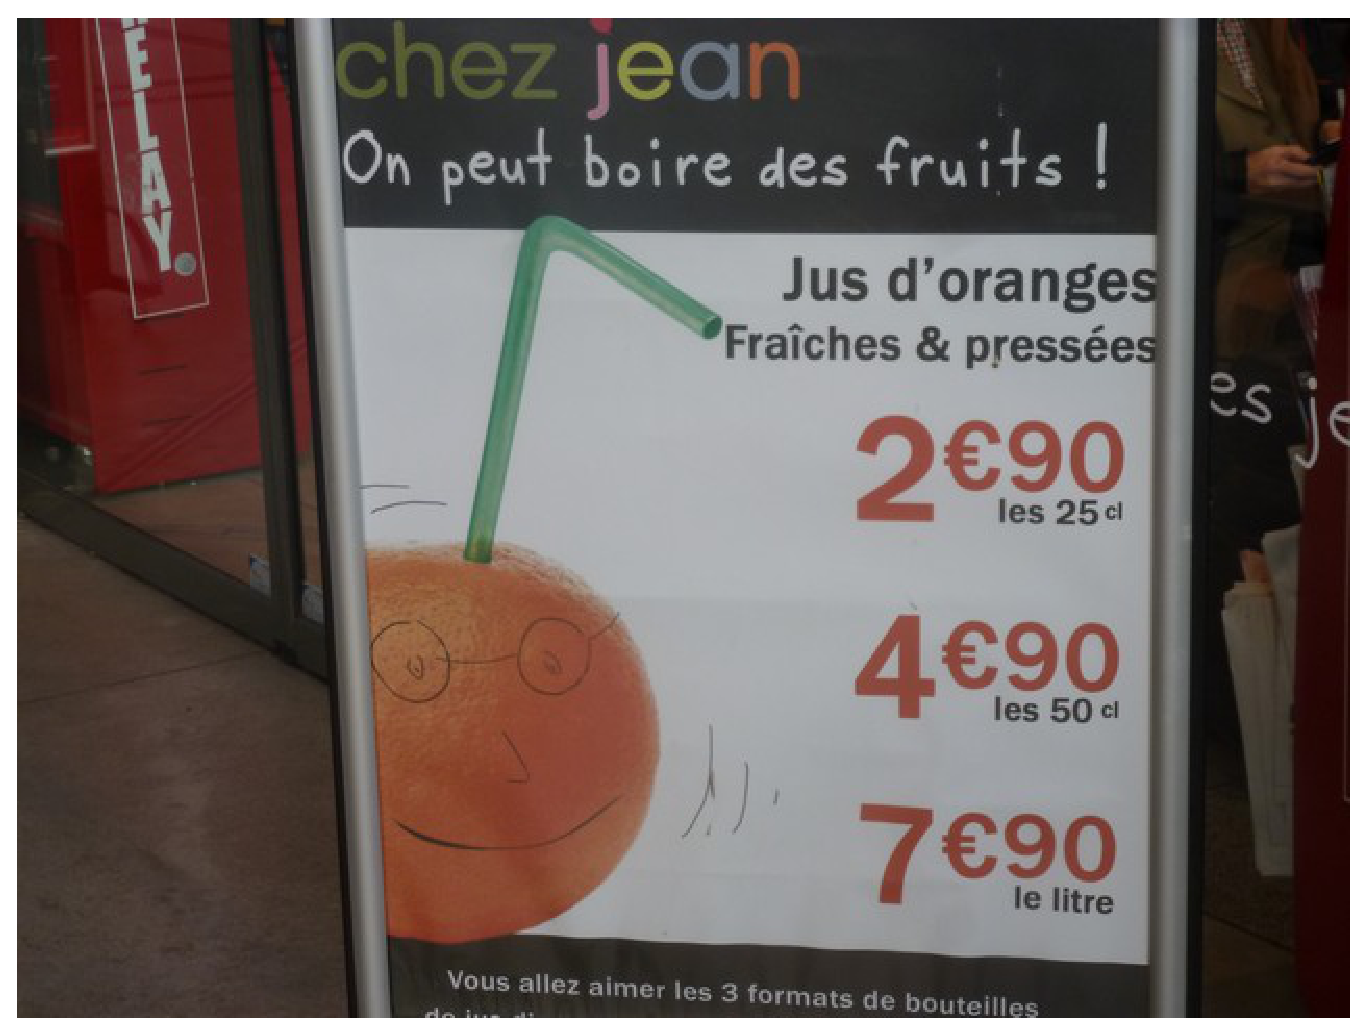
\includegraphics[width=8.4cm]{Transversal/Images/Tra8_crpe_oranges}
\end{minipage}

\bigskip

\begin{minipage}{7cm}
   \fbox{Problème 2} \\ [5mm]
   $\bullet$ Combien vais-je payer si j’achète 3 \oe ufs ? 9~\oe ufs ? 12 \oe ufs ? 24 \oe ufs ? \\
   $\bullet$ Si j’achète 6 \oe ufs, combien est-ce que j’économise par rapport au prix à l’unité ? \\
   $\bullet$ Combien d’\oe ufs au maximum je peux acheter avec 20 \euro ?
\end{minipage}
\qquad
\begin{minipage}{10cm}
      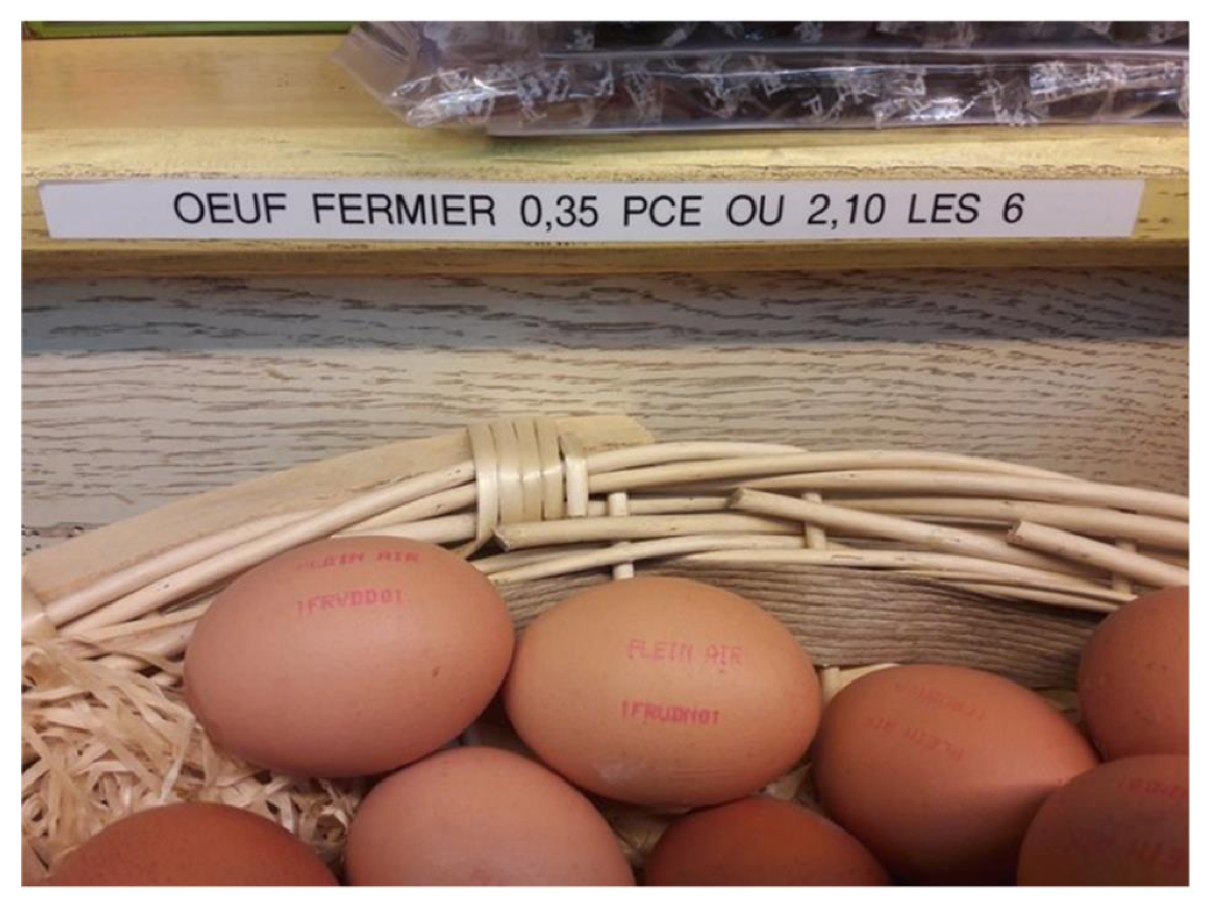
\includegraphics[width=8.4cm]{Transversal/Images/Tra8_crpe_oeufs}
\end{minipage}


%%%%%%%%
\analyses %%%
%%%%%%%%

%%%%%%%%%%%%%%%%%%%%%%%%%%%%%%%%
%\begin{exercice*}[CRPE 1998 Montpellier]
%Le test suivant a été proposé à des élèves de différents niveaux de l'école élémentaire. \\
%Voici quatre segments A, B, C, D ; on veut les agrandir. On a effectué l'agrandissement des segments A et B. \\
%Effectue le même agrandissement pour les segments C et D.
%\begin{center}
%{\psset{unit=0.7}
%\begin{pspicture}(0,0)(10,6.5)
%   \multido{\n=0+0.5}{19}{\psline[linecolor=darkgray](\n,0)(\n,6.5)}
%   \multido{\n=0+0.5}{14}{\psline[linecolor=darkgray](0,\n)(9,\n)} 
%   \psline[linewidth=0.75mm]{|-|}(1,1)(8,1)
%   \rput(0.25,1.25){D}
%   \psline[linewidth=0.75mm]{|-|}(1,2.5)(7,2.5)
%   \rput(0.25,2.75){C}
%   \psline[linewidth=0.75mm]{|-|}(1,4)(4,4)
%   \rput(0.25,4.25){B}
%   \psline[linewidth=0.75mm]{|-|}(1,5.5)(5,5.5)
%   \rput(0.25,5.75){A}
%\end{pspicture}
%\begin{pspicture}(0,0)(13,6.5)
%   \multido{\n=0+0.5}{27}{\psline[linecolor=darkgray](\n,0)(\n,6.5)}
%   \multido{\n=0+0.5}{14}{\psline[linecolor=darkgray](0,\n)(13,\n)} 
%   \psline[linewidth=0.75mm](1,0.75)(1,1.25)
%   \rput(0.25,1.25){D}
%   \psline[linewidth=0.75mm](1,2.25)(1,2.75)
%   \rput(0.25,2.75){C}
%   \psline[linewidth=0.75mm]{|-|}(1,4)(5.5,4)
%   \rput(0.25,4.25){B}
%   \psline[linewidth=0.75mm]{|-|}(1,5.5)(7,5.5)
%   \rput(0.25,5.75){A}
%\end{pspicture}}
%\end{center}
%\underline{Réponses des élèves} (les longueurs sont exprimées en carreaux).
%\begin{center}
%{\renewcommand{\arraystretch}{1.25}
% \begin{tabular}{|c|c|c|}
%      \hline
%      & Longueur du segment C & Longueur du segment D \\
%      \hline
%      élève 1 & 16 & 18 \\
%      \hline
%      élève 2 & 18 & 20 \\
%      \hline
%      élève 3 & 18 & 21 \\
%      \hline
%      élève 4 & 12 & 14 \\
%      \hline
%      élève 5 & 16 & 19 \\
%      \hline
%   \end{tabular}}
%\end{center}
%\begin{enumerate}
%   \item Quelle notion mathématique est principalement mise en jeu dans cet exercice ?
%   \item Donner les principaux paramètres de la situation qui peuvent avoir une influence sur la difficulté de l'exercice.
%   \item Indiquer trois procédures correctes que peuvent utiliser des élèves de CM2 pour répondre.
%   \item Observer les réponses des cinq élèves. Relever les erreurs et émettre une hypothèse sur l'origine de chacune.
%\end{enumerate}
%\end{exercice*}
%
%\begin{corrige}
%\ \\ [-5mm]
%\begin{enumerate}
%   \item Il s'agit d'agrandissements dans le domaine des grandeurs et mesures, qui se caractérise par une relation de {\bf proportionnalité} entre les longueurs des segments correspondants.
%   \item Les paramètres sont les variables didactiques dont le choix des valeurs influe sur les solutions élaborées par les élèves. On peut citer par exemple :
%   \begin{itemize}
%      \item le {\bf rapport} entre les segments données. On a les couples (8,12) pour A, (6,9) pour B, on peut définir le coefficient de proportionnalité qui est $\times$ 1,5 ;
%      \item les {\bf relations} entre les segments dont les agrandissements sont donnés et ceux dont il faut construire les agrandissements : la longueur C est double de la longueur B, celle de D est la somme de celle de A et B ; ces choix ouvrent la possibilité de mettre en \oe uvre les propriétés additives et multiplicatives de la linéarité ;
%      \item le {\bf choix du support} et la position des segments : le support quadrillé sur lequel les segments sont dessinés, en suivant les lignes du quadrillage et s'arrêtant sur des n\oe uds du quadrillage facilite l'évaluation de la longueur de ces segments ;
%      \item le {\bf nombre de segments} donnés : le fait que deux couples soient donnés renforce le repérage de la proportionnalité, favorise la multiplicité des procédures possibles et offre une occasion de repérer que l'ajout d'un même nombre à toutes les longueurs n'est pas pertinent.
%   \end{itemize}
%   \item Procédures possibles pour des élèves de CM2 :
%   \begin{itemize}
%     \item utilisation des propriétés de {\bf linéarité} : multiplicative pour C, dont la longueur est double de celle de B et additivité pour D, dont la longueur est la somme de celles de A et de B.
%       \item utilisation du fait que chaque longueur peut être obtenue en ajoutant à chaque longueur donnée sa moitié (idée de faire une fois et demi), ce qui correspond à une procédure {\bf mixte} (multiplicative et additive) ;
%       \item utilisation du {\bf coefficient de proportionnalité} (1,5) : identification sur les longueurs relatives aux deux couples de segments donnés, puis application aux longueurs des deux autres segments.
%        \end{itemize}
%   \item 
%      {\bf élève 1 :} ajout de 4 aux longueurs de chacun des segments C et D. Obstacle additif, il a repéré que le segment A avait été allongé de 4 carreaux, il fait de même pour les segments C et D. \\
%      {\bf élève 2 :} réponse correcte pour C, erreur pour D, sans doute due au fait que le segment D initial mesure 2 de plus que C, écart reproduit sur les segments agrandis, obstacle additif. \\
%      {\bf élève 3 :} bonne réponse aux deux questions. \\
%      {\bf élève 4 :} simple reproduction des segments C et D donnés. Erreur peut-être due au fait que les segments sont désignés par les mêmes lettres. \\
%      {\bf élève 5 :} pour C, ajout de 4 à la longueur de C comme pour A. Pour D, ajout de 5 à la longueur de D, un peu plus que pour A, peut-être parce que la longueur du segment D est plus longue que celle du segment C. Obstacle additif et éventuellement erreur de calcul et de tracé.
%\end{enumerate}
%\end{corrige}
%
%\bigskip
%
%\begin{exercice*}[CRPE 2014 Sujet 0]
%\textbf{Situation A} -- Le problème ci-dessous a été donné en évaluation à des élèves de cycle 3.
%\begin{center}
%   \fbox{\it à chaque saut, une sauterelle avance de 30 cm. Combien de sauts doit-elle faire pour parcourir 15 mètres ?}
%\end{center}
%\vspace*{-0.5cm}
%\begin{enumerate}
%   \item Dans cet énoncé, qu'est-ce qui indique que la situation est une situation de proportionnalité ?
%   \item Le problème a été proposé à 4 élèves dont les productions sont données page suivante. Pour chacun des 4 élèves.
%   \begin{enumerate}
%      \item Expliquer, en argumentant à partir des traces écrites de l'élève, si la procédure qui semble avoir été utilisée témoigne d'une mise en \oe uvre correcte des propriétés mathématiques de la proportionnalité.
%      \item émettre une hypothèse sur la cause des erreurs éventuelles.
%   \end{enumerate}
%   \item D'un point de vue théorique, cette situation de proportionnalité peut être modélisée par une fonction linéaire du nombre de sauts.
%   \begin{enumerate}
%      \item Expliciter cette fonction.
%      \item Donner la réponse attendue en utilisant cette fonction.
%   \end{enumerate}
%\end{enumerate} 
%
%\vspace*{-1cm}
%\begin{center}
%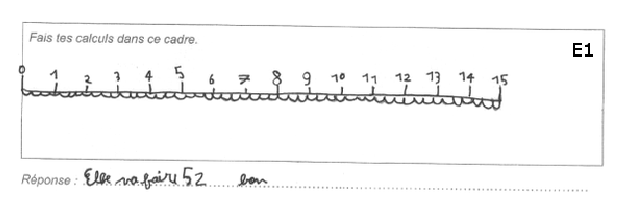
\includegraphics[width=10cm]{Organisation_gestion_donnees_did/Images/Tra8_cours_mousse_E1} \\
%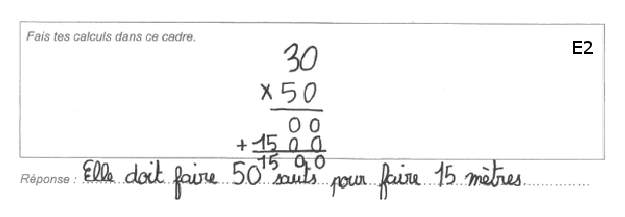
\includegraphics[width=10cm]{Organisation_gestion_donnees_did/Images/Tra8_cours_mousse_E2} \\
%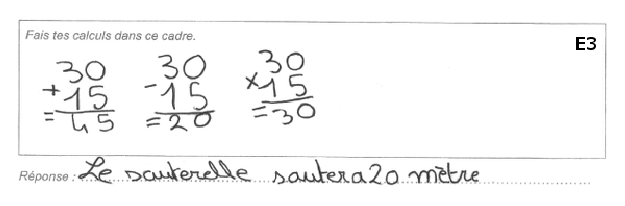
\includegraphics[width=10cm]{Organisation_gestion_donnees_did/Images/Tra8_cours_mousse_E3} \\
%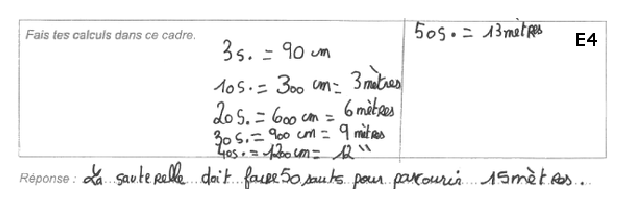
\includegraphics[width=10cm]{Organisation_gestion_donnees_did/Images/Tra8_cours_mousse_E4}
%\end{center}
%
%\textbf{Situation B} -- Le problème ci-dessous a été donné à des élèves à l'entrée en sixième.
%\vspace*{-0.25cm}
%\begin{center}
%   \fbox{\it 6 objets identiques coûtent 150 \euro. Combien coûtent 9 de ces objets ?}
%\end{center}
%\vspace*{-0.75cm}
%\begin{enumerate}
%   \item Dans cet énoncé, qu'est-ce qui indique que la situation est une situation de proportionnalité ?
%   \item D'un point de vue mathématique, qu'est-ce qui différencie cet énoncé du précédent ?
%   \item Proposer trois méthodes possibles pour résoudre cet exercice en cycle 3, et pour chacune expliciter les propriétés mathématiques utilisées.
%\end{enumerate}
%
%\textbf{Situation C} -- En classe de CM2, un professeur propose le travail suivant aux élèves.
%\vspace*{-0.25cm}
%\begin{center}
%\fbox{\begin{minipage}{15cm}
%    {\it Un pavé droit a pour base un carré de côté 2 cm. On fait varier sa hauteur et on s'intéresse à son volume.
%   \begin{enumerate}
%      \item Complète le tableau de valeurs suivant \\
%      \qquad \begin{tabular}{|c|c|c|c|c|c|c|}
%         \hline
%         Hauteur du prisme droit & 2 cm & 3 cm & 4 cm & 5 cm & 6 cm & 10 cm \\
%         \hline
%         Volume du prisme droit& & & & & & \\
%         \hline
%      \end{tabular}
%      \item Place sur la feuille les six points correspondant aux six colonnes du tableau (le professeur a distribué une feuille de papier quadrillé sur laquelle les deux axes gradués d'un repère orthogonal ont été tracés. Sur l'axe des abscisses il a indiqué : hauteur du pavé droit, et sur celui des ordonnées : volume du pavé droit).
%      \item Que constates-tu ? vérifie avec ta règle.
%   \end{enumerate}}
%   \end{minipage}}
%\end{center}
%\vspace*{-0.6cm}
%\begin{enumerate}
%   \item Citer une nouvelle caractérisation de la proportionnalité mise en évidence dans cet exercice.
%   \item Dans cet énoncé, c'est la hauteur du pavé droit qui varie. Si le professeur avait choisi de faire varier la longueur du côté du carré de la base, qu'est-ce que cela aurait changé ? Justifier.
%\end{enumerate} 
%\end{exercice*}
%
%\begin{corrige}
%\textbf{Situation A} \\
%\begin{enumerate}
%   \item Le début de la phrase \og à chaque saut, une sauterelle avance de 30 cm.\fg{} montre une situation de proportionnalité.
%   \item {\bf élève E1.} \\
%   \begin{enumerate}
%      \item Il a représenté une échelle graduée en mètres, régulièrement espacée, puis il a dessiné des \og petits ponts \fg{} représentant les sauts. Enfin, il a compté le nombre de \og petits ponts \fg{}. Il s'agit bien d'une procédure de proportionnalité dans la mesure où chaque saut mesure 30 cm.
%      \item Il aurait pu trouver le résultat exact en ayant construit un axe gradué beaucoup plus précis : en effet, l'axe n'est pas tracé à la règle, et même si les graduations semblent correctement espacées, les \og petits ponts \fg{} sont représentés de manière très peu précise. Il a dû penser que dans un mètre, c'est à dire 100 cm, il y a un peu plus de 3 sauts ($\ucm{30}+\ucm{30}+\ucm{30} =\ucm{90}$ qui est plus petit que \ucm{100}), mais un peu moins de 4 sauts  ($\ucm{30}+\ucm{30}+\ucm{30}+\ucm{30} =\ucm{120}$ qui est plus grand que \ucm{100}). Il a alors dessiné pour chaque graduation un peu plus de 3 petits ponts.
%   \end{enumerate}
%   {\bf élève E2.} \\
%   \begin{enumerate}
%      \item Il a effectué une multiplication exacte qui donne un résultat correct. Il s'agit d'une procédure de proportionnalité puisqu'il utilise le coefficient de proportionnalité (50) pour obtenir son résultat.
%      \item Le résultat est juste, mais on ne sait pas comment l'élève a déterminé le nombre à multiplier par 30 pour obtenir le résultat car il n'a donné aucune trace intermédiaire.  Il est possible qu'il ait utilisé les propriétés d'homogénéité et\slash ou d'additivité du type \og un saut mesure 30 cm, donc 10 sauts mesurent 300 cm\dots \fg.
%   \end{enumerate}
%      {\bf élève E3.} \\
%   \begin{enumerate}
%      \item Il effectue les différents types d'opérations qu'il connait, mis à part la division. Il donne ensuite l'un des résultats qui lui semble peut-être le plus cohérent ? Il n'y a aucune situation de proportionnalité dans ses calculs.
%      \item On peut observer que la compréhension de l'énoncé et de l'utilisation des différentes opérations ne semblent pas être assimilées, les techniques opératoires ne sont pas maitrisées (seule l'addition est juste). La réponse n'est pas non plus en relation avec la question posée. Nous sommes en présence d'un élève qui ne sait pas comment résoudre ce problème, il sait implicitement que la résolution passe par un calcul, mais il ne sait pas lequel.
%   \end{enumerate}
%      {\bf élève E4.} \\
%   \begin{enumerate}
%      \item Il semble utiliser différentes propriétés de la proportionnalité comme la propriété additive (10 sauts mesurent 300 cm, 20 sauts mesurent 600 cm, donc 30 sauts mesurent 900 cm), l'homogénéité (10 sauts mesurent 300 cm, son double 20 sauts mesurent le double de 300 cm) et le coefficient de proportionnalité simple (un saut mesure 30 cm, donc 3 sauts mesurent 3 fois 30 cm) mais on ne connait pas exactement le cheminement pour obtenir ses calculs. Les conversions sont exactes ainsi que la phrase de conclusion.
%      \item Une seule erreur à noter, relevant sûrement d'un faute d'étourderie, l'élève indique que 50 sauts mesurent 13 mètres dans le deuxième cadre de calcul, alors que sa réponse est bien 15 mètres.
%   \end{enumerate}
%   \item
%   \begin{enumerate}
%      \item Il faut tout d'abord harmoniser les unités de mesure pour obtenir un résultat cohérent. Si l'on garde le résultat en cm, alors un saut mesure 30 cm et $x$ saut mesurent $30\times x$ cm. \\
%Soit $y$ le résultat en cm, on a alors $y=30x$ où $x$ est le nombre de sauts effectués. Ceci est bien l'équation d'une fonction linéaire. Cette situation peut être modélisée par la fonction \bm{$f\,:\,x\to30x$.}
%      \item On résout l'équation : $f(x)=1\,500 \Longleftrightarrow 30x=1\,500\Longleftrightarrow \quad x=\dfrac{1\,500}{30} \Longleftrightarrow \quad x=50$. \\
%   \bm{La sauterelle devra effectuer 50 sauts pour parcourir 15 mètres. } \\
%   \end{enumerate}
%\end{enumerate}
%
%\Coupe
%
%\textbf{Situation B} \\
%\begin{enumerate}
%   \item Le fait que les objets soient \og \textbf{identiques} \fg{} indique une situation de proportionnalité.   
%   \item La plus grande différence vient du fait que, dans l'énoncé précédent, on nous donne la valeur d'un seul objet, ce qui simplifie ensuite la procédure à effecteur. Dans ce deuxième énoncé, on nous donne le prix pour 6 objets. Nous sommes donc dans une différence mathématique de l'ordre de la méthode de proportionnalité à utiliser. \\
%Une autre différence résulte dans les unités : en effet, le premier énoncé utilise différentes unités (les centimètres et les mètres) alors que celui-ci n'en utilise qu'une : les euros. Nous sommes donc dans une différence mathématique de l'ordre des conversions.
%   \item \textbf{Méthode 1 :} 6 objets identiques coûtent 150 \euro, donc 3 objets identiques coûtent 75 \euro{} (propriété multiplicative de la linéarité, on prend la moitié des objets, donc la moitié du prix) ; Or, $9=6+3$, donc 9 objets identiques coûtent 150 \euro{}+ 75 \euro{} = 225 \euro{} (propriété additive de la linéarité). \\
%   \textbf{Méthode 2 :} 6 objets identiques coûtent 150 \euro, donc 3 objets identiques coûtent 75 \euro{} (on prend la moitié des objets, donc la moitié du prix) ; donc 9 objets identiques coûtent $3\times75$ \euro{} = 225 \euro{} (on prend le triple des objets, propriété multiplicative de la linéarité uniquement). \\
%   \textbf{Méthode 3 :} 6 objets identiques coûtent 150 \euro, donc 1 objet coûte six fois moins : 150 \euro{} $\div$ 6 = 25 \euro ; et 9 objets identiques coûtent neuf fois plus : $9\times25$ \euro{} = 225 \euro{} (passage par l'unité). \\
%   \textbf{Méthode 4 :} le coefficient de proportionnalité est de 25 (car $6\times25 =150$), donc 9 objets coûtent $225\text{ \euro}$ (utilisation du coefficient de proportionnalité : $9\times25 =225$), notons qu'il est assez peu probable qu'un élève de début de 6\up{ème} utilise cette procédure en raison de la difficulté de \og voir facilement \fg{} le coefficient de proportionnalité. \\
%\end{enumerate}
%
%\textbf{Situation C} \\
%\begin{enumerate}
%   \item Cet exercice permet de mettre en évidence une propriété graphique de la proportionnalité qui est le fait que les points formés par les couples de nombres associés sont alignés sur une droite passant par l'origine du repère.
%   \item Dans le cas d'un pavé droit à base carrée de côté $c$ et de hauteur $h$, on a $\mathcal{V} =c\times c\times h$. \\
%On obtient les deux situations suivantes : \\
%\begin{tabular}{l|l}
%   \textbf{variation de la hauteur $h$ \hspace*{3cm}} & \textbf{variation du côté du carré de base $c$} \\
%   $\mathcal{V} =2\times 2\times h$ & $\mathcal{V} =c\times c\times 2$. \\
%   $\mathcal{V} =4h$ & $\mathcal{V} =2\,c^2$ \\
%\end{tabular} \\
%La première formule $\mathcal{V} =4h$ caractérise bien une situation de proportionnalité puisqu'il s'agit d'une fonction linéaire ; en revanche, la seconde formule $\mathcal{V} =2\,c^2$ ne montre pas une situation de proportionnalité (la fonction obtenue est une parabole, il n'y a pas alignement des points.)
%\end{enumerate}
%\end{corrige}
%
%\bigskip

\begin{exercice}[CRPE 2014 G2]
Un enseignant traite la proportionnalité avec des élèves de cycle 3. \\
{\bf A.} L'enseignant s'interroge sur l'énoncé d'un exercice, pour lequel une phrase (notée [\dots]) reste à préciser :
\begin{center}
\fbox{
\begin{minipage}{12cm}
   {\it Pour une visite au Château de Versailles, la coopérative scolaire doit payer 105 \euro{} pour une classe de 15 élèves de CE1. Mais un groupe de 20 élèves de CE2 se joint finalement à cette classe. [\dots] \\
  Combien la coopérative devra-t-elle payer en tout ?}
\end{minipage}}
\end{center}
\begin{enumerate}
   \item Proposer une phrase complétant l'énoncé pour que cette situation soit sans ambiguïté une situation de proportionnalité.
   \item Proposer une phrase complétant l'énoncé pour que cette situation ne soit pas une situation de proportionnalité.
\end{enumerate}
{\bf B.} L'enseignant propose l'institutionnalisation de la proportionnalité ci-dessous à partir de celle proposée dans le manuel  \og Outils pour les maths \fg{} - CM1 - Magnard - édition 2011 :
\begin{center}
   \fbox{
   \begin{minipage}{12cm}
   {\it {\bf On reconnaît une situation de proportionnalité lorsque le rapport entre les nombres ne change pas.} \\
   $\bullet$ Exemple 1 : {\bf 1 kg de pêches coûte 3 \euro.} \\ [1mm]
   \hspace*{2cm}
     \begin{tabular}{|l|C{0.5}|C{0.5}|C{0.5}|}
         \hline
         Nombre de kg de pêches & 1 & 2 & 5 \\
         \hline
         Prix en \euro & 3 & 6 & 15 \\
         \hline
      \end{tabular}
   \smallskip\\
   Le prix est proportionnel à la masse. \\
   Pour trouver le prix, il faut multiplier par le même nombre (par 3). \\
   $\bullet$ Exemple 2 : {\bf 4 gâteaux coûtent 6 \euro.} \\
   Pour trouver le prix de 8 gâteaux, je calcule le double $\rightarrow 6\times2 =12$ \euro. \\
   Pour trouver le prix de 2 gâteaux, je calcule la moitié $\rightarrow 6\div2 =3$ \euro. \\
    $\bullet$ Exemple 3 : {\bf 1 stylo coûte 2 \euro, 3 stylos coûtent 5 \euro, 6 stylos coûtent 6 \euro}. \\
    Dans cette situation, 3 stylos ne coûtent pas {\bf 3 fois plus cher} qu'un stylo, 6 stylos ne coûtent pas 6 fois plus cher. \\
    {\bf Cette situation n'est pas proportionnelle.}}
\end{minipage}}
\end{center}
\begin{enumerate}
   \item Quelle propriété caractéristique de la proportionnalité le traitement de l'exemple 1 illustre-t-il ?
   \item Quelle propriété caractéristique de la proportionnalité le traitement de l'exemple 2 illustre-t-il ?
   \item Dans cet extrait de manuel, l'expression \og rapport entre les nombres \fg{} désigne dans le traitement des exemples 1 et 2, des coefficients jouant des rôles différents.
Expliciter ces différents rôles.
   \item Quelle propriété caractéristique de la proportionnalité est utilisée dans le traitement de l'exemple 3 ? Donner une autre façon de mettre en évidence que la situation n'est pas une situation de proportionnalité, faisant appel à une autre propriété caractéristique.
\end{enumerate}
{\bf C.} L'enseignant propose un autre exercice :
\begin{center}
\fbox{
\begin{minipage}{12cm}
   {\it Lorsque je fais une mousse au chocolat pour 8 personnes, j'utilise 6 \oe ufs. \newline
   Quand je fais une mousse au chocolat pour 12 personnes, j'utilise 9 \oe ufs. \newline
   Combien faudra-t-il d\oe ufs si je fais une mousse au chocolat pour 20 personnes ?}
\end{minipage}}
\end{center}
Analyser les quatre productions des élèves page suivante, en précisant les propriétés mathématiques implicitement mobilisées.
\begin{center}
   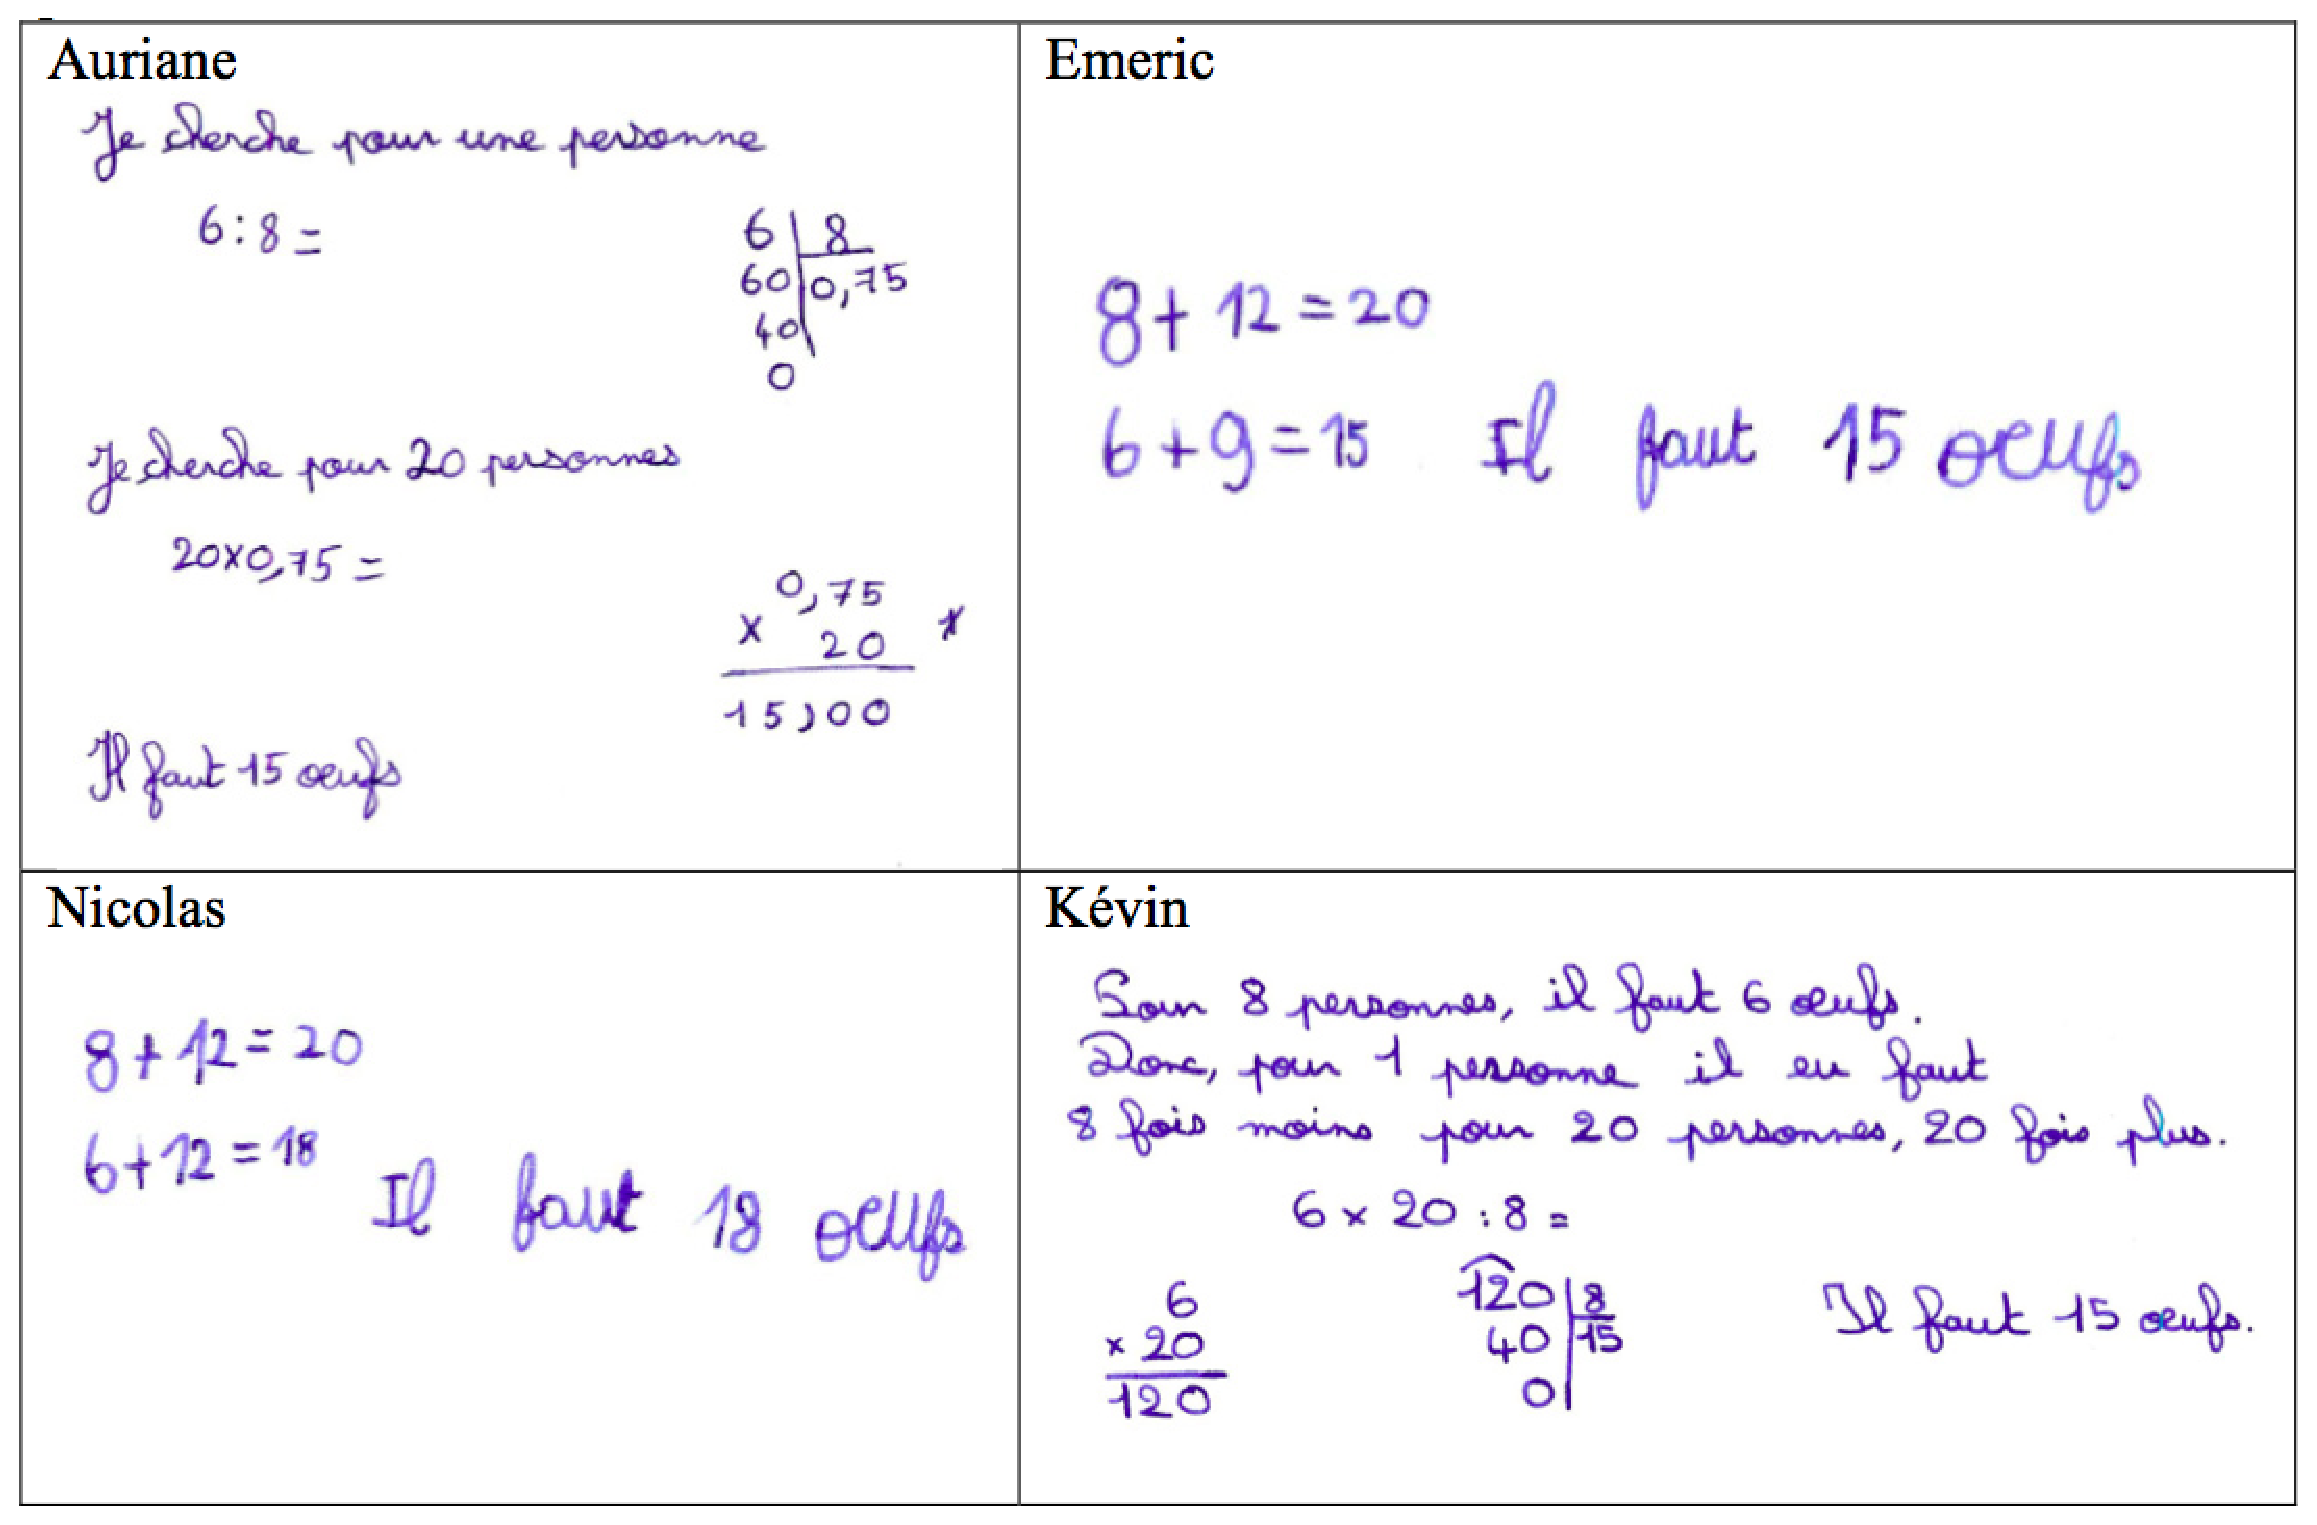
\includegraphics[width=15cm]{Transversal/Images/Tra8_analyse_mousse}
\end{center}
{\bf D.} L'enseignant propose un dernier exercice :
\begin{center}
\fbox{
\begin{minipage}{12cm}
   {\it Dans une ville, il y a deux médiathèques. \newline
   Le service culturel de cette municipalité effectue un recensement des fonds d'ouvrages de chaque établissement. à cette fin, les documentalistes ont relevé les éléments suivants :
   \begin{itemize}
      \item à la médiathèque Jean Jaurès, on peut trouver 5\,000 ouvrages dont 40\,\% de romans ;
      \item à la médiathèque George Sand, on peut trouver 4\,000 ouvrages dont 60\,\% de romans.
   \end{itemize}
   Calculer le pourcentage de romans au sein du service culturel de la ville.}
\end{minipage}}
\end{center}
\begin{enumerate}
   \item Pourquoi cet exercice s'inscrit-il dans une séquence d'apprentissage traitant de la proportionnalité ? à quel niveau du cycle 3 va-t-on de préférence proposer cet exercice ?
   \item Après une phase de recherche individuelle, l'enseignant organise une phase de mise en commun. \\
   Paul dit : \og J'ai trouvé 50\,\% parce que c'est exactement entre 40\,\% et 60\,\% \fg.
   \begin{enumerate}
      \item Quelle erreur de raisonnement Paul commet-il ?
      \item Par quel nombre faudrait-il remplacer 5000 pour que 50\,\% soit la bonne réponse ? Justifier.
   \end{enumerate}
\end{enumerate}
\end{exercice}

\begin{corrige}
{\bf A.} 
\begin{enumerate}
   \item On pourrait compléter, par exemple, par \og La coopérative avait acheté 25 tickets d'entrée, tous aux même prix, elle en achète 20 autres au même tarif \fg.
   \item \og Sachant qu'il y a une réduction de 2 \euro{} par ticket à partir du vingtième élève. \fg{} \\
\end{enumerate}

{\bf B.} 
\begin{enumerate}
   \item L'exemple 1 illustre l'utilisation du {\bf coefficient de proportionnalité} (toutes les valeurs d'une même grandeur sont obtenues en multipliant les valeurs de l'autre grandeur par le même nombre).
   \item L'exemple 2 illustre l'utilisation de la {\bf linéarité multiplicative}, ou homogénéité (quand l'une des grandeurs est multipliée ou divisée par un nombre, l'autre grandeur est multipliée ou divisée par le même nombre).
   \item Dans l'exemple 1, le rapport est le coefficient de proportionnalité. Il est le même pour toutes les données. Dans l'exemple 2, il s'agit d'un coefficient de linéarité, ou coefficient scalaire entre deux grandeurs identiques.
   \item Il s'agit ici de la propriété multiplicative de la linéarité, qui n'est pas vérifiée. \\
   On aurait également pu remarquer que 6 stylos, c'est 3 stylos + 3 stylos. Or le prix n'est pas égal à 5 \euro{} + 5 \euro{}, la situation n'est donc pas proportionnelle en vertu de la propriété additive de la linéarité qui n'est pas vérifiée. \\
\end{enumerate}

{\bf C.} {\bf Auriane} effectue un {\bf passage par l'unité} : elle calcule le nombre d'\oe ufs nécessaires pour une personne, puis pour 20 personnes. Son raisonnement, sa rédaction et son résultat sont corrects. \\
   {\bf émeric} utilise utilise la propriété {\bf additive} de la linéarité : pour 20 personnes (8+12), il faut 15 \oe ufs (6+9). Son raisonnement et son résultat sont corrects. \\
   {\bf Nicolas} se trompe dans son raisonnement : il ajoute une même grandeur (12 personnes) à la fois aux 8 personnes (ce qui est cohérent), mais aussi au nombre d'\oe ufs ! Son résultat est donc faux. Il est possible qu'il ait souhaité utilisé la propriété additive de la linéarité, qu'il ne maîtrise pas. \\
   {\bf Kévin} effectue le {\bf passage par l'unité}. Son raisonnement, sa rédaction et son résultat son corrects. En revanche, il n'effectue pas les opérations dans l'ordre de son raisonnement écrit : il commence par multiplier par 20 (le nombre de personnes) au lieu de diviser par 6 (le nombre d'\oe ufs). Cependant, étant donné la commutativité de la multiplication et de la division, le résultat demeure juste. \\

{\bf D.} 
\begin{enumerate}
   \item La notion de pourcentage relève de la proportionnalité : il s'agit du nombre qui aurait été proportionnellement obtenu si l'effectif avait été de 100. Il sera donné plutôt en 6\up{e} puisque, seuls les pourcentages simples (25\,\%, 50\,\%\dots) en lien avec les fractions doivent être acquis à l'école.
   \item
   \begin{enumerate}
      \item Paul effectue la moyenne des deux pourcentages. Ce qui est faux dans la plupart des cas. C'est juste uniquement lorsque l'effectif de départ est strictement le même dans les deux situations.
      \item Pour que 50\,\% soit la bonne réponse, il faudrait que les deux médiathèques disposent du même nombre de livres, soit 4\,000 livres à la bibliothèque jean Jaurès.
   \end{enumerate}
\end{enumerate}
\end{corrige}

\bigskip

\begin{exercice}[CRPE 2016 G2]
Un enseignant propose le problème suivant à ses élèves de cycle 3 :
\begin{center}
\fbox{
\begin{minipage}{12cm}
   Nicolas a acheté 2 kg de pommes. Il a payé 4 \euro. \\
   Léo a acheté la même variété de pommes dans le même magasin. Il a payé 5 \euro. \\
   Quelle masse de pommes a-t-il achetée ?
\end{minipage}}
\end{center}
Proposer trois procédures, attendues d' élèves de cycle 3, pour résoudre ce problème, l'une au moins ne nécessitant pas le recours aux nombres décimaux.
\end{exercice}

\begin{corrige}
   \begin{itemize}
       \item {\bf Linéarité mixte, multiplicative puis additive :} \\
          \begin{tabular}{p{7cm}c|cp{7.5cm}}
             Avec utilisation des décimaux
             & & &
             Sans utilisation des décimaux \\
             \hline
             Pour 4 \euro, on a 2 kg de pommes, donc pour 1 \euro, on a 0,5 kg de pommes et pour 5 \euro{} = 4 \euro + 1 \euro, on a 2 kg + 0,5 kg  = 2,5 kg de pommes.
             & & &
             Pour 4 \euro, on a 2\,000 g de pommes, donc pour 1 \euro, on a 500 g de pommes et pour 5 \euro{} = 4 \euro + 1 \euro, on a 2\,000 g + 500 g  = 2\,500 g de pommes.
          \end{tabular}
      \item {\bf Passage par l'unité :} \\
          \begin{tabular}{p{7cm}c|cp{7cm}}
             Avec utilisation des décimaux
             & & &
             Sans utilisation des décimaux \\
             \hline
             2 kg de pommes coûtent 4 \euro, donc pour 1 \euro, on a 0,5 kg (2 kg$\div$4) et pour 5 \euro, on a 2,5~kg ($5\times0,5\text{ kg} =2,5$ kg).
             & & &
             2\,000 g de pommes coûtent 4 \euro, donc, pour 1 \euro, on a 500 g (2\,000 g$\div$4) et pour 5 \euro, on a 2\,500 g ($5\times500\text{ g} =2\,500$ g).
      \end{tabular}
   \end{itemize}

\Coupe

   \begin{itemize}
      \item {\bf Coefficient de proportionnalité :} \\
   pour passer de 2 à 4, on multiplie par 2, il s'agit du coefficient de proportionnalité. Donc, pour obtenir un prix de 5 \euro, il faut 2,5 kg de pommes ($2,5\times2 =5$).
   \end{itemize}
\end{corrige}

\bigskip

\begin{exercice}[CRPE 2017 G1]
L’exercice ci-dessous est extrait des évaluations nationales CM2 de 2008.
\begin{center}
\fbox{
\begin{minipage}{12cm}
   {\it Pour faire des crêpes pour 6 personnes, il faut :
   \begin{itemize}
      \item 250 g de farine ;
      \item 1 litre de lait ;
      \item 4 oeufs ;
      \item 1 cuillerée à soupe d’huile ;
      \item 2 pincées de sel.
   \end{itemize}
Calcule la quantité de chacun des ingrédients nécessaire pour faire des crêpes pour 9 personnes.}
\end{minipage}}
\end{center}
Voici les productions de trois élèves :
\begin{center}
   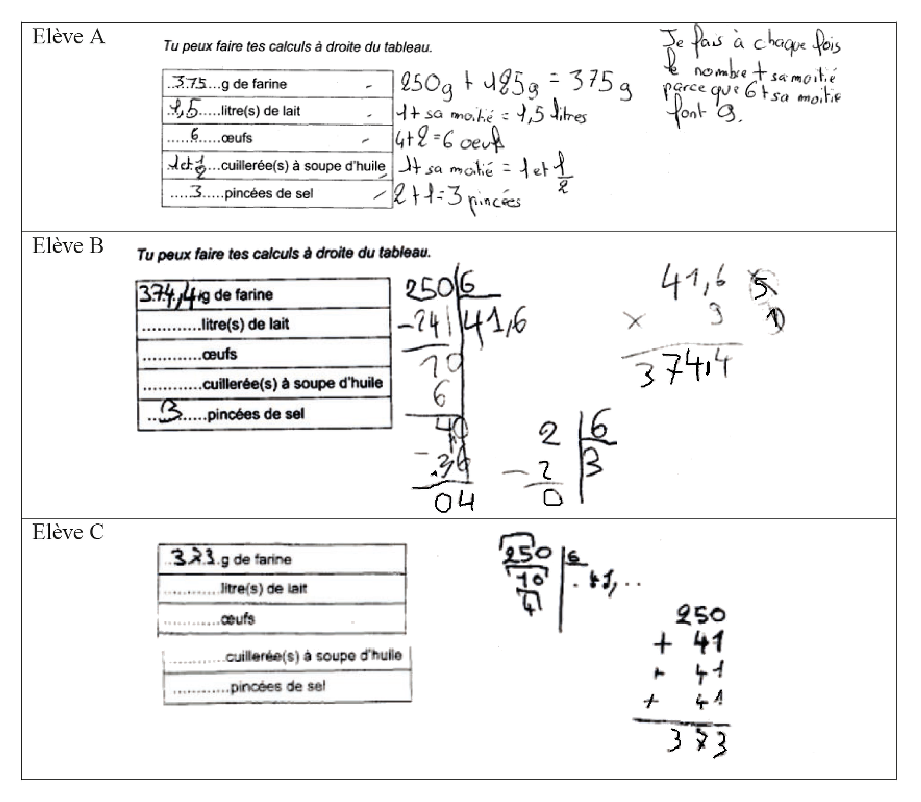
\includegraphics[width=15cm]{Transversal/Images/Tra8_analyse_crepes}
\end{center}
\begin{enumerate}
   \item Quelle est la principale notion du programme sur laquelle cet exercice permet de revenir ?
   \item Expliciter les procédures utilisées pour le calcul de la masse de farine nécessaire par chacun des élèves A, B et C.
   \item En quoi le choix de 300 g de farine nécessaires au lieu de 250 g aurait-il pu modifier les procédures proposées par les élèves ?
\end{enumerate}
\end{exercice}

\begin{corrige}
\ \\ [-5mm]
\begin{enumerate}
   \item La principale notion travaillée ici est la \textbf{proportionnalité} dans le cadre de la résolution d'un problème.
   \item Procédures des élèves A, B et C.
   \begin{itemize}
      \item L'\textbf{élève A} utilise une procédure mixte de linéarité : il utilise la propriété additive de la linéarité pour dire que 9 personnes, c'est 6 personnes plus 3 personnes, et la propriété multiplicative de la linéarité pour dire que 3 personnes, c'est la moitié de 6 personnes. Pour chacune de ces quantités, il associe la quantité d'ingrédients correspondant. Sa procédure est juste, son résultat également. On pourrait éventuellement lui demander de préciser les unités dans ses calculs.
      \item L'\textbf{élève B} utilise le passage par l'unité : il calcule la masse de farine pour une personne puis, il multiplie par 9 qui est le nombre de personnes. La procédure est correcte, mais il trouve une valeur approchée, donc son résultat est erroné (le problème ici est que la valeur obtenue par la division de 250 par 6 est une valeur approchée puisque $\frac{250}{6}$ est un nombre rationnel non décimal). Pour les pincées de sel, il commence par poser sa division mais ne va pas au bout : son résultat est juste, mais l'opération est fausse, peut-être parce qu'il l'a en fait trouvé par une autre méthode. Il n'a pas le temps de calculer toutes les quantités.
      \item L'\textbf{élève C} semble vouloir utiliser le passage par l'unité en posant la division euclidienne de 250 par 6 sans résultats intermédiaires. Pourtant, il pose la virgule et met des pointillés pour exprimer le fait que \og ça continue \fg{} et il obtient 41 qui correspond à la masse de farine en gramme pour une personne. Ensuite, on veut la masse pour 9 personnes alors qu'on a à l'origine la masse pour 6 personnes, soit 3 personnes de plus, donc il additionne la masse de farine à trois fois le quotient entier (41) trouvé grâce à son opération ce qui est un raisonnement juste mais approximatif. Il trouve 373 qui est une valeur assez proche du résultat, mais fausse.
   \end{itemize}
   \item 300 est un multiple de 6, ce qui est avantageux au niveau du calcul : pour une procédure par passage à l'unité, le résultat de la division est un entier, donc l'élève B par exemple arriverait à un résultat juste. Mais ces nombres permettent aussi une autre procédure, celle de la recherche du coefficient de proportionnalité permettant de passer de 6 personnes à une masse de 300 g qui est un coefficient relativement simple (50). Ce coefficient pouvait être trouvé par un calcul mental, par un procédure type essais-erreurs ou par une division.
\end{enumerate}
\end{corrige}

\bigskip

\begin{exercice}[CRPE 2018 G3]
Une enseignante de CM2 propose l’exercice suivant en classe de CM2.
\begin{center}
\fbox{
   \begin{minipage}{12cm}
      Une boîte contient des dragées toutes identiques. \\
      120 dragées pèsent 360 g. \\
      Combien pèsent 30 dragées ?
   \end{minipage}
}
\end{center}
\begin{enumerate}
  \item Proposer trois procédures pouvant être utilisées par les élèves pour résoudre cet exercice, en explicitant à chaque fois chacun des calculs effectués pour trouver le résultat attendu.
   \item L’enseignante veut vérifier la maitrise de la procédure dite de retour à l’unité par les élèves. Elle souhaite garder la même forme d’exercice en modifiant les nombres en jeu dans l’énoncé pour contraindre, ou au moins encourager vivement, les élèves à utiliser cette procédure. Proposer un énoncé modifié qu’elle pourrait soumettre à ses élèves.
\end{enumerate}
\end{exercice}

\begin{corrige}
\ \\ [-5mm]
\begin{enumerate}
   \item On peut utiliser les procédures suivantes :
      \begin{itemize}
         \item On a 30 dragées, soit 4 fois moins de dragées puisque 120 dragées $\div$ 4 = 30 dragées donc, la masse de 30 dragées est 4 fois plus petite et vaut 360 g $\div$ 4 = 90 g. \\
            Utilisation d'un coefficient scalaire (coefficient de linéarité multiplicative) égal à 1/4.
         \item $120\times3 =360$ donc, 30$\times$3 =90. La masse de 30 dragées est de 90 g. \\
            Utilisation du coefficient de proportionnalité qui vaut 30.
         \item 120 dragées pèsent 360 g donc, une dragée pèse $\dfrac{360\text{ g}}{120} =3$ g. \\
            D'où 30 dragées pèsent $30\times3$ g = 90 g. Utilisation du passage par l'unité.
      \end{itemize}
   \item Pour \og espérer \fg{} une procédure par retour à l'unité, il faut que les autres procédures soient moins évidentes. Or, les nombres en jeu sont propices à l'utilisation d'un coefficient scalaire (un quart) ou de proportionnalité (30) qui sont simples à obtenir mentalement. On pourrait donc, par exemple, modifier l'énoncé de la façon suivante : 
   \medskip
   \fbox{
      \begin{minipage}{12.5cm}
         Une boîte contient des dragées toutes identiques. 120 dragées pèsent 270 g. \\
         Combien pèsent 32 dragées ?
      \end{minipage}} \\
      Le coefficient scalaire devient 3,75 et le coefficient de proportionnalité 2,25 qui ne sont pas \og simples \fg. 
\end{enumerate}
\end{corrige}

\bigskip

\begin{exercice}[CRPE 2018 G2]
Un enseignant propose la situation suivante en cycle 3 :
\begin{center}
\fbox{
   \begin{minipage}{5cm}
      Consignes données oralement : \\ [5mm]
      \og Voici un puzzle carré. \\
      Vous allez devoir refaire le même puzzle mais en plus grand. Il faudra le reconstituer exactement avec les pièces agrandies. \\
      Le segment de 4 cm devra mesurer 6 cm sur votre puzzle agrandi. \\
     Le compte-rendu de vos recherches sera présenté sous la forme d’une affiche \fg.
   \end{minipage}
   \qquad
   \begin{minipage}{8.5cm}
   \psset{unit=0.6}
   \begin{pspicture}(-1.5,-1)(12.5,12)
      \psframe(0,0)(11,11)
      \psline(4,0)(4,9)(11,9)
      \psline(11,2)(4,9)
      \psline(6,11)(0,5)
      \psline(6,0)(6,7)
      {\scriptsize
         \rput(12,6){7 cm}
         \rput(12,1){2 cm}
         \rput(12,10.){2 cm}
         \rput(8.5,11.5){5 cm}
         \rput(3,11.5){6 cm}
         \rput(-1,8.){6 cm}
         \rput(-1,2.5){5 cm}
         \rput(2,-0.5){4 cm}
         \rput(5,-0.5){2 cm}
         \rput(8.5,-0.5){5 cm}
         \rput(3,4){9 cm}
         \rput(7,3){7 cm}
         \rput(8,9.5){7 cm}
      }
      \rput(2,9){A}
      \rput(9.5,10){B}
      \rput(2,2.5){C}
      \rput(5,4){D}
      \rput(8.5,2){E}
      \rput(9,7){F}
   \end{pspicture}
   \end{minipage}
}
\end{center}
{\it Modalités de mise en \oe uvre : le professeur demande aux élèves de travailler par groupes de quatre, de s’accorder sur la procédure à adopter pour agrandir les éléments du puzzle, de se répartir la construction des pièces en faisant leurs calculs individuellement puis d’assembler les morceaux pour reconstituer le puzzle agrandi.} \\
\begin{enumerate}
   \item Quel champ mathématique cette situation permet-elle de travailler ?
   \item Analyser les différentes stratégies mises en oeuvre en pointant les réussites et les erreurs des groupes ayant produit les affiches 1, 2 et 3.
   \item Dans la mesure du possible, indiquer les procédures utilisées pour déterminer chacune des valeurs trouvées par le groupe ayant produit l’affiche 4.
\end{enumerate}
\begin{center}
   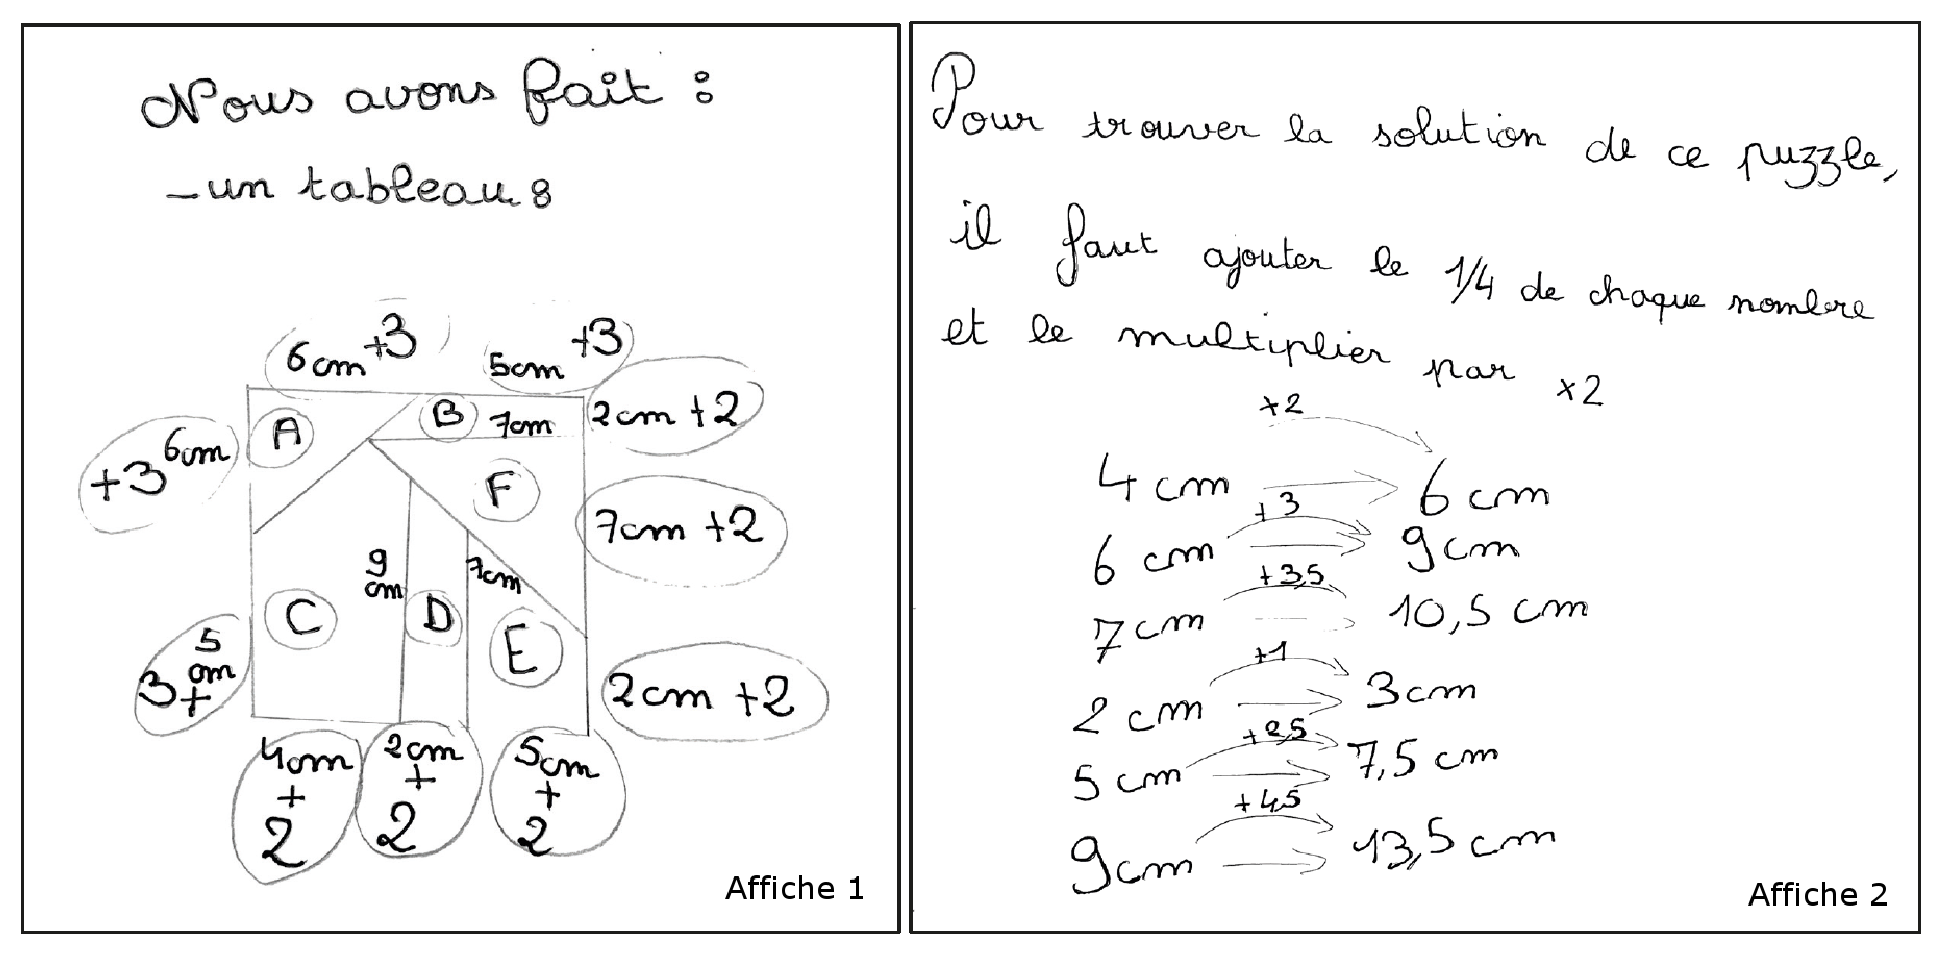
\includegraphics[width=17cm]{Transversal/Images/Tra8_analyse_puzzle1} \\
   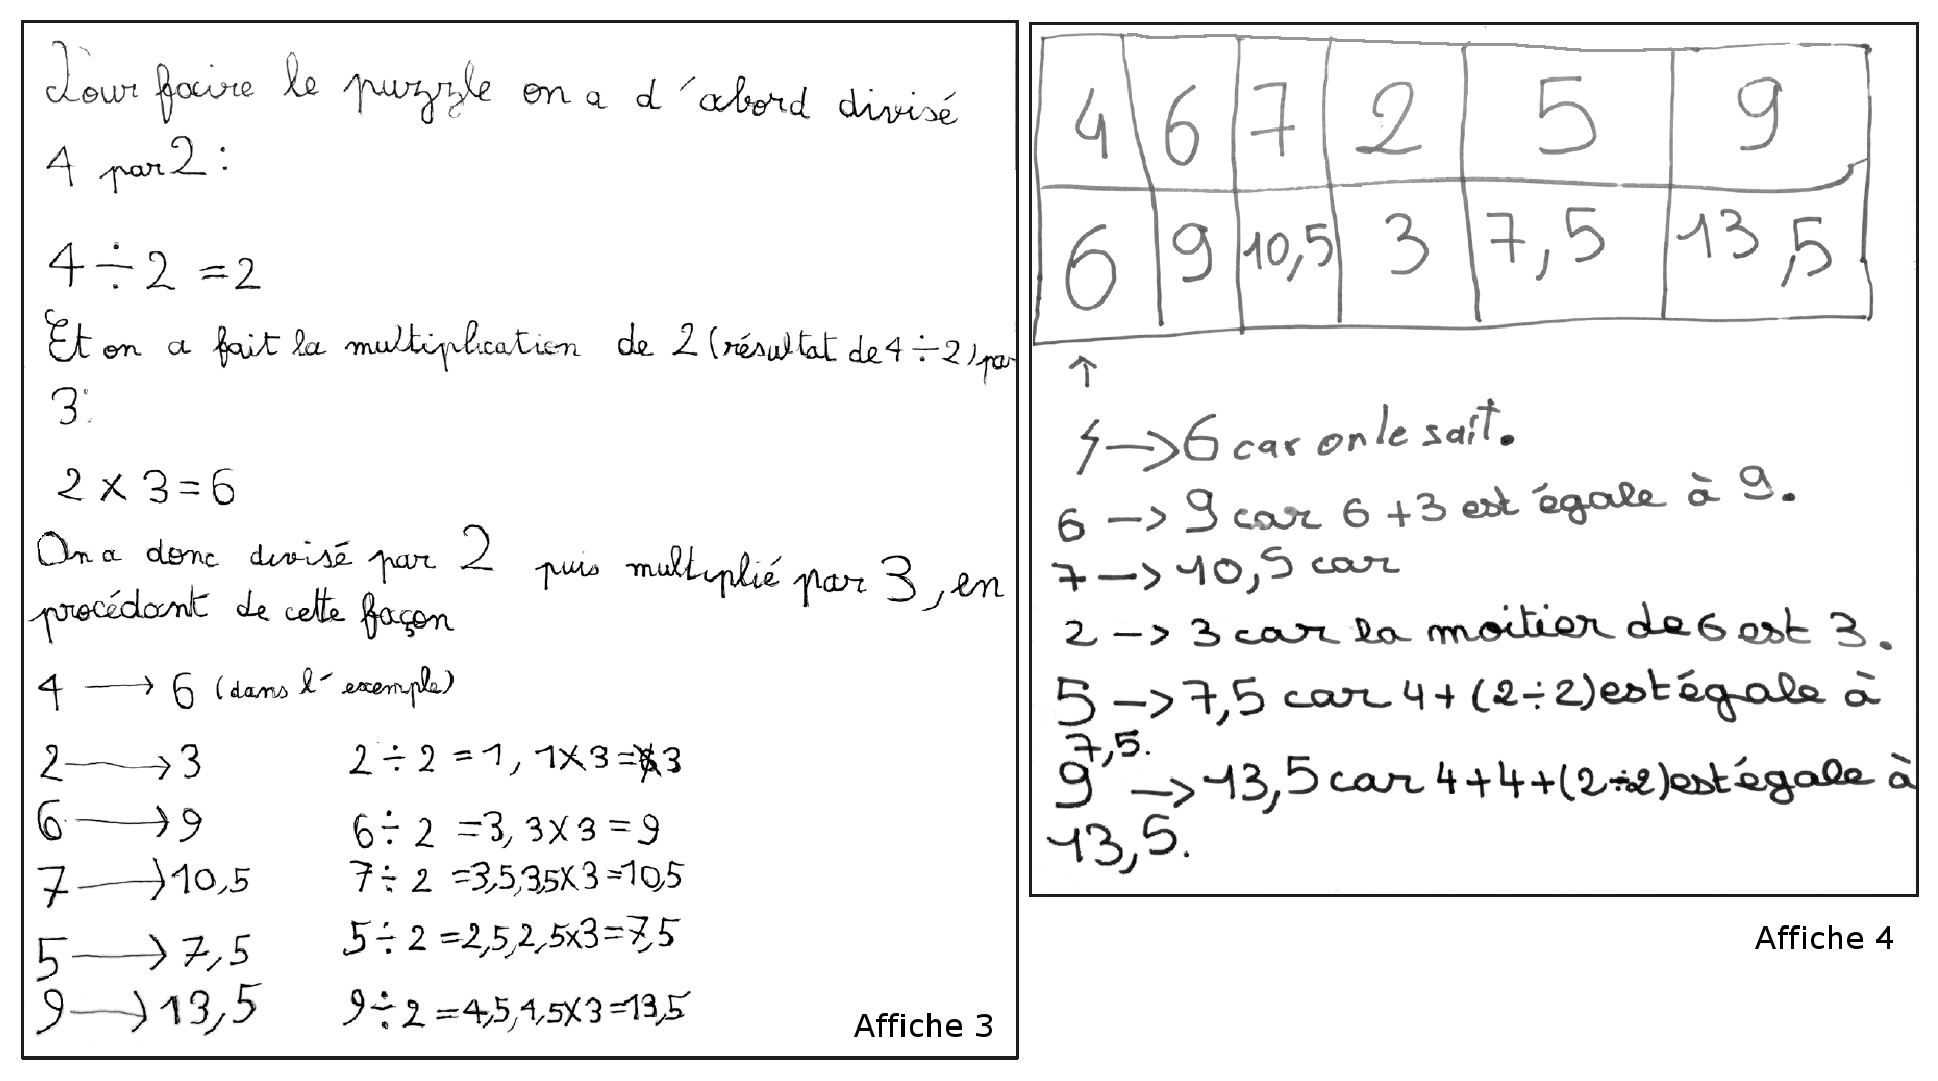
\includegraphics[width=17cm]{Transversal/Images/Tra8_analyse_puzzle2}
\end{center}
\end{exercice}

\begin{corrige}
\ \\ [-5mm]
   \begin{enumerate}
      \item Cette situation permet de travailler le champ multiplicatif puisqu'il s'agit d'une activité d'agrandissement. Plus particulièrement, la situation se situe dans le thème transversal de la proportionnalité dans le domaine des grandeurs et mesures. 
      \item Analyse des trois premières affiches :
         \begin{itemize}
            \item {\bf Affiche 1.} Les élèves ont \og vu \fg{} que 6 cm, c'est 4 cm + 2 cm. Ils ont donc ajouté 2 cm à toutes les mesures du côté droit et du bas du carré. Pour le haut et le côté gauche, ils ont ajouté 3 cm, peut-être parce que les valeurs d'origine à augmenter (5 cm et 6 cm) sont plus grandes, donc il faut ajouter un peu plus que 2 cm. On remarque toutefois que l'agrandissement est le même pour toutes les mesures d'un même côté, y compris pour 7 cm qui est plus grand que 6 cm. \\
            Réussites : ils ont su modéliser la situation par un schéma, ils ont repéré qu'il ne fallait pas toujours ajouter le même nombre. \\
            Erreurs : ils ont commis l'erreur classique consistant à penser qu'augmenter une mesure, c'est ajouter un même nombre, c'est à dire effectuer une addition alors que l'on se situe dans le champ multiplicatif. Les valeurs à l'intérieur du carré n'ont pas été agrandies (oubli ?).
           \item {\bf Affiche 2.} Les élèves ont remarqué qu'ajouter 2 cm à 4 cm, c'est ajouter deux fois 1 cm qui est le quart de 4~cm, c'est à dire, en langage mathématique : 6 cm = 4 cm + $\dfrac14\times$ 4 cm. Ils utilisent les propriétés de linéarité mixte (additive et multiplicative). \\
           Réussites : ils ont su modéliser la situation en donnant toutes les mesures nécessaires pour l'agrandissement du puzzle, ils ont trouvé les bons résultats par un raisonnement tout à fait pertinent. \\
           Erreur : la phrase d'explication est un peu litigieuse car elle laisse penser qu'il faut ajouter le quart de la valeur d'origine (par exemple 4 cm + 1 cm = 5 cm) puis multiplier ce nombre par 2 (2$\times$5 cm = 10 cm). Il aurait été préférable d'écrire par exemple \og il faut prendre le quart de chaque nombre, le multiplier par 2, puis ajouter le nombre obtenu au nombre de départ \fg.
            \item {\bf Affiche 3.} Ils ont utilisé les propriétés de linéarité multiplicative appliquées aux valeurs données dans l'énoncé (4 cm devient 6 cm) en prenant les deux coefficients scalaires $\dfrac12$  et 3 : 6, c'est 3 fois 2 et 2, c'est 4 divisé par 2. Ensuite, ils ont appliqué ces coefficients à chacune des mesures du dessin. \\
      Réussites : explication claire de la procédure, calculs corrects sans erreur d'écriture y compris pour les nombres décimaux. \\
      Pas d'erreur.
         \end{itemize}
      \item Procédures utilisées pour l'affiche 4 :
         \begin{itemize}
            \item \bm{$4\to6$} : reprise de l'énoncé.
            \item \bm{$6\to9$} : on peut penser que les élèves ont ajouté la moitié de 6 à 9 qui est 3 en vertu de ce qu'ils ont fait par la suite.
            \item \bm{$7\to10,5$} : pas d'explication.
            \item \bm{$2\to3$} : par analogie avec la correspondance $4\to6$, 2 étant la moitié de 4, il faut calculer la moitié de 6 qui est 3. Ils ont utilisé implicitement la propriété de linéarité multiplicative de la proportionnalité.
            \item \bm{$5\to7,5$} : 5 c'est 4 + 1 soit 4 + 2$\div$2 donc, les élèves utilisent une procédure mixte utilisant la linéarité additive et multiplicative. Ils appliquent alors cette procédure pour passer de 5 à 7,5 : pour 4 cm, l'agrandissement vaut 6 cm et pour 2 cm, il est de 3 cm, donc pour 1 cm il est de 1,5 cm et pour 5 cm on a donc 6 cm + 1,5 cm = 7,5 cm.
            \item \bm{$9\to13,5$} : même procédure que précédemment en utilisant la décomposition $9 = 4 + 4 + 1$ soit $4 + 4 + 2\div2$. Pour 4 cm on a 6 cm et pour 2 cm on a 3 cm, donc pour 9 cm, on a 6 cm + 6 cm + 3 cm $\div$ 2 = 13,5 cm.
         \end{itemize}
   \end{enumerate}
\end{corrige}


%%%%%%%%%
\Recreation %%%
%%%%%%%%%

\setcounter{exercice}{0}

\begin{exercice*}[Découverte de la proportionnalité]
   Cette activité d'introduction à la proportionnalité est issue du manuel \og maths au CM1 \fg, édition Accès, pages 138-142. Il s'agit de la séance 1 et dure 45 minutes environ. La compétence travaillée est : reconnaître et résoudre un problème de  proportionnalité en utilisant une procédure de linéarité. \medskip
   
   {\bf -- étape 1 : Recherche} \\
   Les élèves prennent connaissance du problème : \\
     {\it \og Madline assemble des cubes identiques pour construire une muraille devant son château-fort. \\
     Elle construit une muraille où tous les cubes sont alignés comme dans le schéma ci-dessous. \fg
     \begin{center}
        \begin{pspicture}(0,-0.4)(4,1)
           \multido{\n=0+1}{4}{\rput(\n,0){\psframe(0,0)(1,1)}}
           \psline{<->}(0,-0.3)(4,-0.3)
           \rput(2,-0.6){\ucm{12}}
        \end{pspicture}
     \end{center}
     Avec 4 cubes assemblés, sa muraille mesure \ucm{12}. \\
     Combien mesurera la muraille si elle associe 8 cubes ? 12 cubes ? 20 cubes ?} \\
     Consigne : Répondez aux trois questions sans utiliser de règle graduée, ni de matériel. \medskip
     
     {\bf -- étape 2 : Mise en commun} \\
     Inciter les élèves à comparer les différentes procédures et faire prendre conscience qu'en fonction des nombres en jeu, certaines sont plus efficaces que d'autres. \\
     Ici, les procédures de linéarité additive et multiplicative sont possibles. On notera que la procédure de passage à l'unité relève du CM2, et celle du coefficient de proportionnalité de la 6\up{e}. \medskip
     
     {\bf -- étape 3 : Validation par manipulation} \\
     Certains élèves sont confrontés à un obstacle cognitif car ils n'envisagent que des relations additives entre nombres. Ce qui les conduit à répondre 18 cm pour 8 cubes, puisqu'on est passé de 4 cubes à \ucm{12} en \og ajoutant \fg{} 8. On leur fait alors valider en utilisant du matériel comme des cubes de 3 cm de côté, ou de carrés de côté \ucm{3}. Cela permet à certains élèves de confronter leurs résultats, éventuellement erronés, à la réalité par validation expérimentale. \medskip
     
     {\bf -- étape 4 : Institutionnalisation} \\ [1mm]
        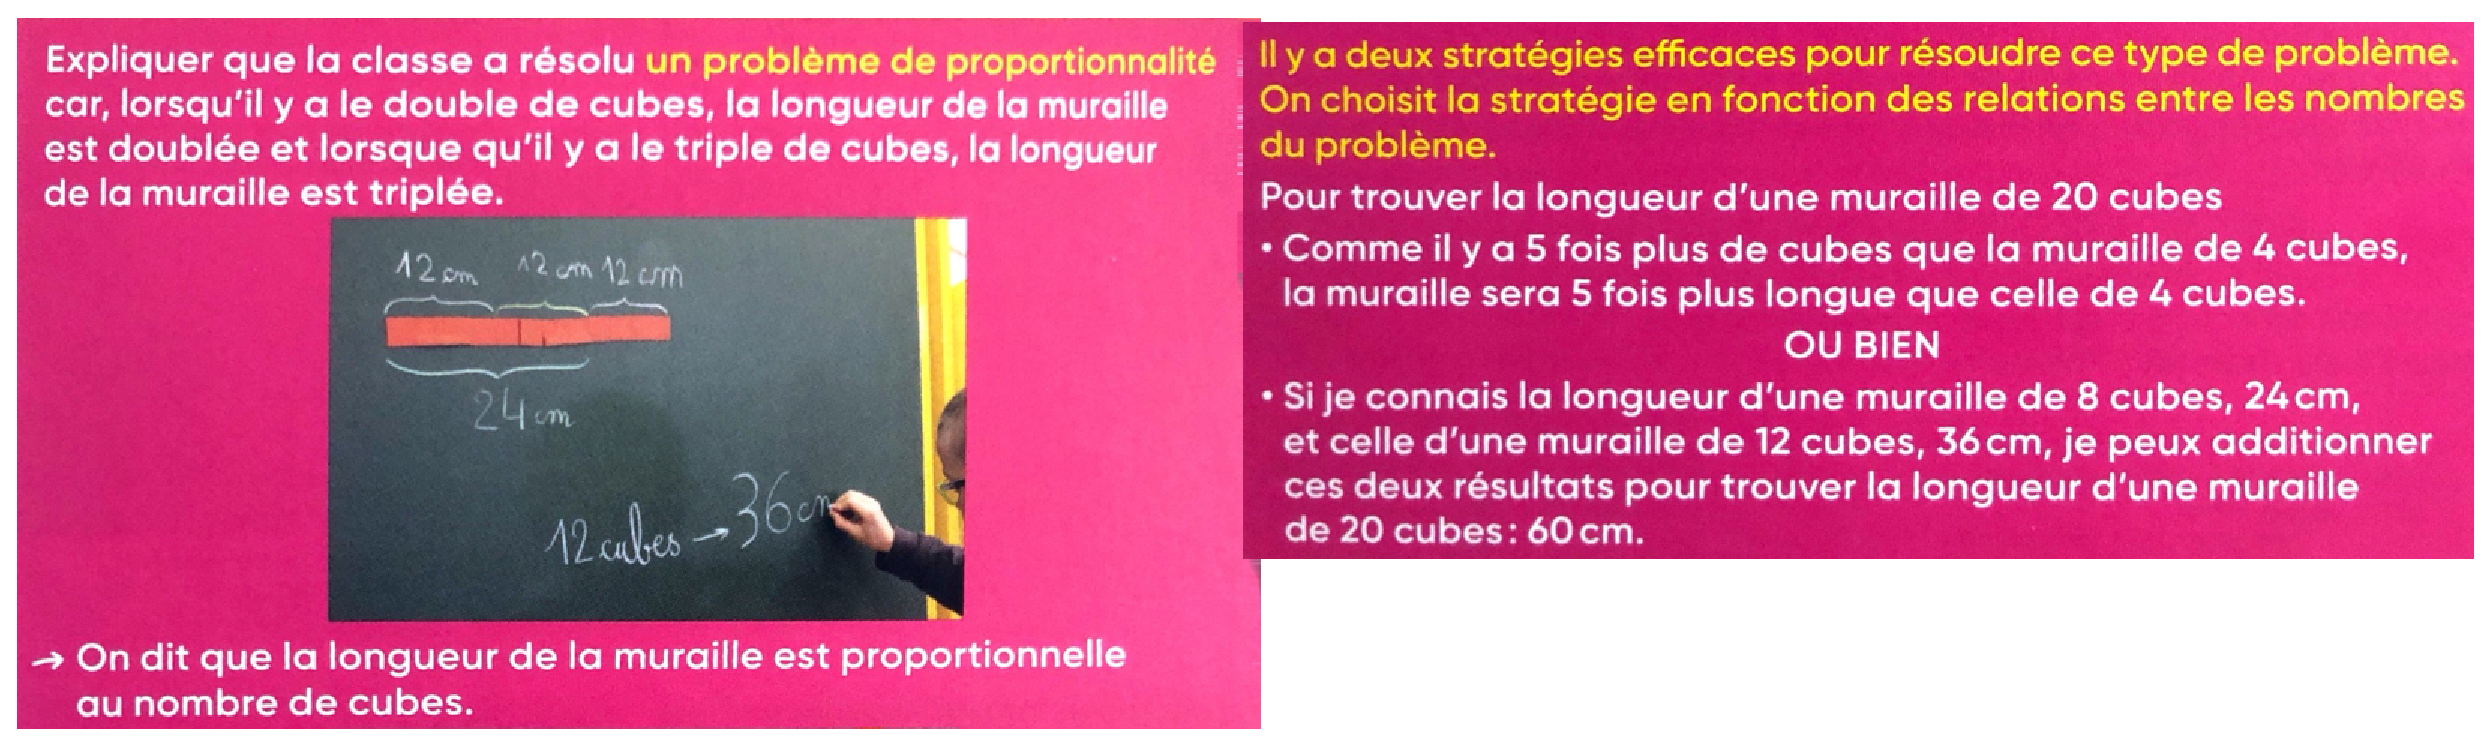
\includegraphics[width=17cm]{Transversal/Images/Tra8_activite_proportionnalite_cubes} \\
        
     La séance suivante propose de travailler la même situation en faisant v varier les données numériques : 4 cubes dont la mesure totale vaut 10 cm, puis 5 cm.
     \begin{center}
        \begin{pspicture}(0,-0.1)(4,1)
           \multido{\n=0+1}{4}{\rput(\n,0){\psframe(0,0)(1,1)}}
           \psline{<->}(0,-0.3)(4,-0.3)
           \rput(2,-0.6){\ucm{10}}
        \end{pspicture}
        \begin{pspicture}(-2,-0.1)(4,1)
           \multido{\n=0+1}{4}{\rput(\n,0){\psframe(0,0)(1,1)}}
           \psline{<->}(0,-0.3)(4,-0.3)
           \rput(2,-0.6){\ucm{5}}
        \end{pspicture}
     \end{center}
\end{exercice*}


\begin{exercice*}[Le puzzle de Brousseau\dots{} adapté !] %%%
   Cette activité est issue du document éduscol [edu3] et propose une adaptation du puzzle de Brousseau : \\
   \href{http://cache.media.education.gouv.fr/file/Proportionnalite/22/5/RA16_C3_MATH_PROPO_PUZZLE_614225.pdf}{\og Résoudre des problèmes de proportionnalité au cycle 3. Activité : Puzzle \fg}.
   
   \begin{minipage}{10cm}
      {\bf énoncé} \\
         Présenter l’activité en parlant d’agrandir la figure. Ne pas parler de proportionnalité à ce stade. \\
         {\it Agrandis les 3 pièces de la figure de façon à ce que les segments mesurant \ucm{2} mesurent finalement \ucm{6}.} \\
         Les dimensions de la figures peuvent être données, ou être mesurées directement sur la figure. \\ [1mm]
      {\bf Modalités de travail} \\
         Par groupe de trois élèves. Chaque élève a une pièce du puzzle à construire. La recherche est tout d'abord individuelle, puis le groupe échange au sujet des procédures. Ces différentes procédures seront reproduites sur une affiche de groupe puis affichées.
   \end{minipage}
   \qquad
   \begin{minipage}{6cm}
      \begin{pspicture}(0,-0.3)(6,6.3)
         \psset{fillstyle=solid,linewidth=0.8mm}
         \psframe[fillcolor=yellow](0,0)(2,4)
         \rput(1,0.35){\ucm{2}}
         \rput{-90}(0.3,2){\ucm{4}}
         \psframe[fillcolor=green](2,0)(6,4)
         \rput(4,0.35){\ucm{4}}
         \rput{90}(5.7,2){\ucm{4}}
         \psframe[fillcolor=orange](0,4)(6,6)
         \rput{-90}(0.3,5){\ucm{2}}
         \rput(3,5.65){\ucm{6}}
      \end{pspicture}
   \end{minipage}
      
   {\bf Critères de réussite} \\
   Condition nécéssaire : l’assemblage des 3 nouvelles pièces constitue à nouveau un carré. \\
   Le carré a pour côté \ucm{18}. \smallskip
   
   {\bf Difficultés prévisibles} \\
   Les élèves risquent d’utiliser des procédures éronées (ajout ou retrait d'un même nombre aux longueurs initiales). \\
   -- En ajoutant \ucm{4} a toutes les mesures, la figure obtenue n'est pas un carré. \\
   -- Avec cette même procédure, ils peuvent aussi \og s'arranger \fg{} pour qua la dernière pièce produise un carré. \smallskip
   
   {\bf Variables didactiques} \\
   -- Proposer différents coefficients d’agrandissement/réduction : 0,5 ; 1,5 ; 2\dots \\
   -- Varier le nombre de pièces, la forme des pièces. \smallskip
   
   {\bf Institutionnalisation} \\
   Diverses phrases peuvent être notées dans les cahiers, par exemple : \\
   \og Une figure agrandie conserve la même forme que la figure initiale. \fg \\
   \og Pour agrandir une figure, il faut multiplier toutes les longueurs par un même nombre. \fg   
   \begin{center}
      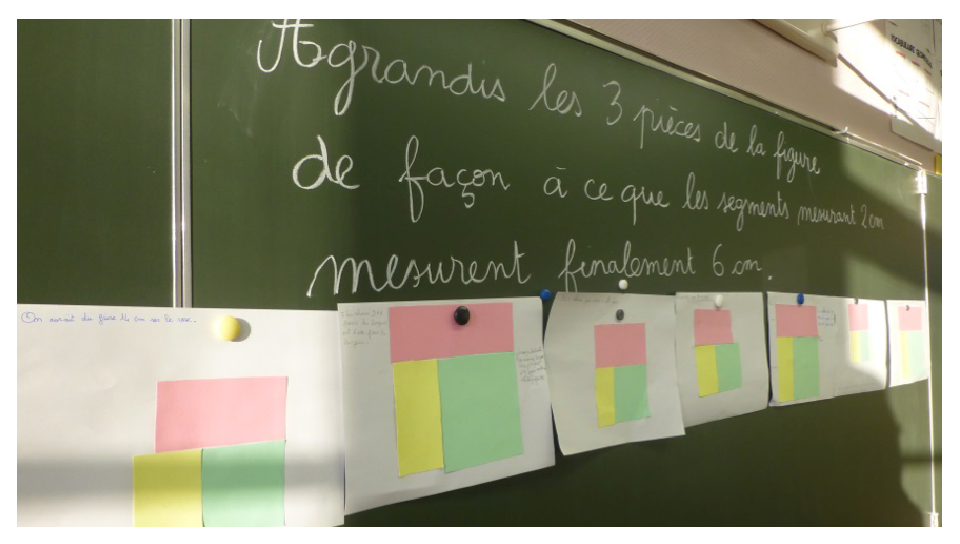
\includegraphics[width=12cm]{Transversal/Images/Tra8_activite_brousseau_adapte}
   \end{center}
\end{exercice*}

